% !TeX spellcheck = en_GB
\documentclass[12pt, a4paper, titlepage, oneside, final]{book}
\usepackage[a4paper, top=30mm, right=25mm, bottom=30mm, left=35mm]{geometry}
%\usepackage{showframe}

\usepackage[utf8]{inputenc}			% utf-8, bitches
\usepackage[T1]{fontenc}			% das Trennen der Umlaute
\usepackage[ngerman,english]{babel}	% word wrapping

\usepackage{parskip}				% makes paragraph spacing nicer
\usepackage{setspace}				% more spacing control
%\setstretch{1.25}

\tolerance 1800
\hbadness 1800
\widowpenalty=10000
\clubpenalty=10000
\displaywidowpenalty=10000
\emergencystretch 1.5em
\raggedbottom

\usepackage[breaklinks,hidelinks]{hyperref}		% links

\usepackage{xspace}					% intelligent spacing after words, usefull for shortcut coammnds
\usepackage{graphicx}				% better graphics support
\usepackage{color}					% enables support for using different colors
\usepackage{csquotes}				% show quotes

\usepackage{comment}
\usepackage{caption}
\usepackage{float}					% better positioning for graphics, tables, etc.
%\usepackage{tabu}					% better tables -> unmaintained?
\usepackage{booktabs}				% improvements to LaTeX tables
\usepackage{tabularx}				% better tables
\usepackage{multirow}				% for cells spanning multiple rows
\usepackage{multicol}				% seems to be necessary for multirow?
\usepackage{calc}					% enables calculations in heights and stuff
\usepackage{wrapfig}				% figures on the side
\usepackage{subcaption}				% captions for subfigures
\usepackage{pdfpages}				% include whole pdfs as pages

\usepackage[title,toc,page]{appendix}		% appendix environment
\usepackage{listings}				% source code listings
%usepackage{longtable}				% multipage tables
%usepackage{array}					% enables the user of m{} and b{} in tables
%usepackage{multirow}				% allow multiple rows

%usepackage{pdflscape}				% produces landscape pages (landscape env)

\usepackage{amssymb}				% math
\usepackage{amsmath}				% more math
\usepackage{textgreek}				% allows for greek chars
\usepackage{xfrac}					% tilted fractions using \sfrac
\usepackage[style=iso]{datetime2}	% date format, that makes sense to everybody

\usepackage[acronym,toc,shortcuts]{glossaries}	% Glossary and Acronym support

\usepackage[backend=bibtex, style=authoryear,
	citestyle=authoryear, sorting=ynt,
	sortcites=true, block=none,	indexing=true,
	citereset=none, isbn=true,
	url=true, doi=true, natbib=false,
	hyperref=true]{biblatex}					% even better citation support
\addbibresource{bas-sec.bib}
\addbibresource{standards.bib}

%
\usepackage{ccicons}				% icons for the creative commons licenses

%
\usepackage{hyperxmp}				% pdf meta information
\hypersetup{
	pdfauthor={Martin Peters},
	pdfauthortitle={Master Student},
	pdfcreator={},
	pdflang={en},
	pdfkeywords={Building Automation, KNX, netflow},
	pdftype={Text},
	pdfcopyright={Copyright (C) 2017/2018, Martin Peters.},
	pdflicenseurl={}
}

% ------------------------------------------------------------------------------
% Shortcuts
% 
\definecolor{pink}{rgb}{1,0,1}
\definecolor{red}{rgb}{1,0,0}
\definecolor{green}{rgb}{0,1,0}

%\newcommand{\hint}[1]{{\color{pink}#1}}
\newcommand{\hint}[1]{}

%\newcommand{\alert}[1]{{\color{red}#1}}
\newcommand{\alert}[1]{}

%\newcommand{\todo}[1]{{\color{green}#1}}
\newcommand{\todo}[1]{}

% Shortcut file


% ------------------------------------------------------------------------------
% Context shortcuts
% 

\newcommand{\hvac}{HVAC\xspace}
\newcommand{\knx}{KNX\xspace}
\newcommand{\lonworks}{LonWorks\xspace}
\newcommand{\bacnet}{BACnet\xspace}

% ------------------------------------------------------------------------------
% Helper functions
% 
\newcommand{\code}[1]{\texttt{#1}}


% ------------------------------------------------------------------------------
% Glossary
% 
\makeglossaries
% ------------------------------------------------------------------------------
% Glossary
% 

% TODO apply something like https://tex.stackexchange.com/a/8951 where acronoyms should also be a glossary entry

% BAS stuff
\newacronym[plural=BAS,firstplural=Building Automation Sytems (BAS)]{bas}{BAS}{Building Automation System}
\newacronym{hvac}{HVAC}{heating, ventilation, and air conditioning}

\newacronym{eib}{EIB}{European Installation Bus}
\newglossaryentry{lon}{name={LonWorks},description={LonWorks}}
\newglossaryentry{bac}{name={BACnet},description={BACnet}}

\newacronym{pir}{PIR}{Passive Infrared Sensor}

% KNX terminology
\newacronym{apci}{APCI}{Application Layer Protocol Control Information}
\newacronym{tpci}{TPCI}{Transport Layer Protocol Control Information}
\newacronym{csmaca}{CSMA/CA}{Carrier Sense Multiple Access / Collision Avoidance}
\newacronym[plural=DPT,firstplural=Datapoint Types (DPT)]{dpt}{DPT}{Datapoint Type}
\newacronym{s-al}{S-AL}{Secure Application Layer}

\newglossaryentry{knx}{name={KNX},description={KNX or Konnex}}
\newglossaryentry{knx-assoc}{name={KNX Association},description={\todo{knx assoc}}}
\newglossaryentry{telegram}{name={Telegram},description={\gls{knx} Packet}}
\newglossaryentry{hops}{name={hop count},description={\todo{hop count}}}
\newglossaryentry{ets}{name={ETS},description={\todo{ETS}}}

% network stuff
\newacronym{ip}{IP}{Internet Protocol}
\newacronym{ids}{IDS}{Intrusion Detection System}
\newacronym{ipfix}{IPFIX}{IP Flow Information eXport}

\newglossaryentry{netflow}{name={Netflow},description={Cisco Netflow is a protocol to perform flow analysis. \textcite[cf.][]{Claise2004}}}

\newglossaryentry{osi}{name={OSI},description={The Open Systems Interconnection Model is a reference model for network protocols, providing an layered view}}

% ML stuff
\newglossaryentry{vect}{name={vector space},description={}}
\newglossaryentry{fvect}{name={feature vector},description={}}

\newacronym[plural=SVM,firstplural=Support Vector Machines (SVM)]{svm}{SVM}{Support Vector Machine}
\newacronym{lof}{LOF}{Local Outlier Factor}
\newacronym{knn}{kNN}{k-Neareast Neighbour}
\newacronym{aakr}{AAKR}{Autoassociative Kernel Regression}
\newacronym{sprt}{SPRT}{Sequential Probability Ratio Test}
\newacronym{ripper}{RIPPER}{Repeated Incremental Pruning to Produce Error Reduction}

% other stuff
\newglossaryentry{py}{name={Python},description={Interpreted Programming Language}}
\newglossaryentry{influxdb}{name={InfluxDB},description={NoSQL time series database}}
\newglossaryentry{idbmeasurement}{name={measurement},plural={measurements},description={An InfluxDB measurement is comparable to a table in relational databases. It contains the timestamp and tags as indecies and fields as data}} %\url{https://docs.influxdata.com/influxdb/v1.4/concepts/key_concepts/#measurement}
\newglossaryentry{grafana}{name={Grafana},description={Open Source time series visualisation and monitoring dashboard}}
\newglossaryentry{rabbitmq}{name={RabbitMQ},description={Open Source message passing server, implementing \gls{amqp}. \\\url{https://www.rabbitmq.com/}}}
\newglossaryentry{lib-click}{name={\code{click}},description={Python package for creating beautiful command line interfaces in a composable way with as little code as necessary. \url{http://click.pocoo.org/6/}}}
\newglossaryentry{baos}{name={KNX BAOS},description={Protocol communicate with \gls{knx} modules developed by Weinzierl Engineering. \url{https://www.weinzierl.de/index.php/en/}}}
\newglossaryentry{lib-pika}{name={\code{pika}},description={Pure Python implementation of the \gls{amqp} 0-9-1 protocol. \\\url{https://pika.readthedocs.io/}}}
\newglossaryentry{json}{name={JSON},description={JavaScript Object Notation is a lightweight data-interchange format}}
\newglossaryentry{unixts}{name={Unix timestamp},description={Timestamp encoded with the (milli-)seconds since \alert{1970-01-01}}}

\newacronym{amqp}{AMQP}{Advanced Message Queuing Protocol}
\newacronym{gil}{GIL}{global interpreter lock}
%\newglossaryentry{gil}{name={GIL},description={Global Interpreter Lock. A mechanism used by the default CPython implementation to ensure that Python bytecode is only executed by one thread at a time}}

\newacronym{scada}{SCADA}{Supervisory Control and Data Acquisition}
\newacronym{ics}{ICS}{Industrial Control Systems}

% stats stuff
\newacronym{pmf}{PMF}{propability mass function}

% crypto
\newacronym{aes}{AES}{Advanced Encryption Standard}
\newacronym{ctr}{CTR}{Counter mode}
\newacronym{ccm}{CCM}{Counter with CBC-MAC}

% attacks
\newacronym{dos}{DoS}{Denial of Service}


% ------------------------------------------------------------------------------
% Titel
% 
\newcommand{\thedate}{2017-03-21}					% TODO change before handing in
\newcommand{\theauthor}{Martin Peters}
\newcommand{\thetitle}{Analysis of Distributed In-Band Monitoring Messages for Field Bus Networks in Building Automation Systems}

\title{\thetitle\\[24pt]
	\small Chair for Information and Communication Services\\[-3pt]
	\small University of Rostock}
\author{\theauthor}
\date{\thedate}
%
% ------------------------------------------------------------------------------

\begin{document}
	% begin with no page numbering
	\pagenumbering{gobble}
	% title
	%\maketitle
	% TitelSeite
\begin{titlepage}

	\begin{center}
		
		\hrule
		\vspace{0.5cm}
		\LARGE {\bfseries \thetitle}
		\vspace{0.5cm}
		\hrule
		
		\vspace{0.8cm}
		\Large {Master Thesis}\\
		\vspace{1.0cm}
		\large {University of Rostock\\
		Faculty of Computer Science and Electrical Engineering\\
		Institute of Computer Science\\
		Chair for Information and Communication Services}
		
		%\vspace{0.8cm}
		\vfill
		
\includegraphics[width=7cm]{style/UNI-Logo.pdf}
		%\vspace{0.8cm}
		
	\end{center}
	
	\vfill
	\large
	\begin{tabular}{lcl}
		Submitted by: &&  \theauthor \\
		Matriculation Number: && 212206972\\
		Born at: && 1993-09-30 in Schwerin\\
		First Reviewer: && Prof. Dr. rer. nat. habil. Clemens H. Cap\\
		Second Reviewer: && Prof. Dr.-Ing. habil. Gero Mühl\\
		Supervisor: && Dr.-Ing. Thomas Mundt\\
		Submission Date: && \thedate
	\end{tabular}
	\normalsize
	
	
\end{titlepage}
	%
	% compiling info
	~ \vfill
	\begin{flushright}
		\tiny \noindent
		{\normalsize \href{http://creativecommons.org/licenses/by-sa/4.0/}{\ccbysa}} \\*[0.5em]
		This work is licensed under a \href{http://creativecommons.org/licenses/by-sa/4.0/}{Creative Commons\\%*[-1em]
		Attribution-ShareAlike 4.0 International License}. \\
		The license of the supplementary material especially source code\\%*[-1em]
		may differ. Please refer to the respective LICENSE files.\\
		\LaTeX ~compiled at \DTMnow
	\end{flushright}
	\pagebreak
	%
	% --------------------------------------------------------------------------
	%
	% begin with roman page numbering
	\clearpage
	\setcounter{page}{1}
	\pagenumbering{roman}
	% the toc
	\pdfbookmark[1]{\contentsname}{Contents}
	\tableofcontents
	% the lof
	\listoffigures\addcontentsline{toc}{chapter}{List of Figures}
	% the lot
	\listoftables\addcontentsline{toc}{chapter}{List of Tables}
	
	% --------------------------------------------------------------------------
	% begin of actual document
	%
	% begin new page numbering
	\newpage
	\pagenumbering{arabic}
	\setstretch{1.25}
	
	\chapter{Introduction}
	\label{sec:intro}
	% !TeX spellcheck = en_US
\section{Motivation}
\begin{itemize}
	\item "[...] the overall concerns are the internal threat (accidental) and the increasing presence of connected devices, many insecure by design, in and around ICS environments." \parencite[p.~9]{Gregory-Brown2017}
	\item "The threat from nearly every vector identified by ICS security practitioners can be reduced by detailed monitoring of ICS network traffic6 in a manner that provides visibility into both process anomalies and security anomalies on the control network, in some cases establishing control points limiting access to different zones of your network" \parencite[p.~10]{Gregory-Brown2017}
	\item "4 out of 10 ICS security practitioners lack visibility or sufficient supporting intelligence into their ICS networks" \parencite[p.~13]{Gregory-Brown2017}
\end{itemize}

\section{Scope of this work}

\section{Negative scope of this work}
\begin{itemize}
	\item only \knx
	\item no real impl of the agent, focus only on collector
	\item no optimization for high throughput
	\item no infrastructure for deploy'n'forget (no automatic learning etc.)
		\subitem this is research, installation requires manual steps
	\item no classification of intrusion?
	\item well aware of privacy implications, but not part of this work
\end{itemize}

\section{Research Questions}

\begin{enumerate}
	\item \enquote{[...] anomaly detection methods seem especially applicable to SCADA system security which are characterized by routine and repetitious activities.} \parencite{Yang2006} Is it also a good fit for BAS? Does it make sense?
	\item How can anomaly detection identify different attack vectors in BAS:
		\subitem new devices
		\subitem (high) traffic load
		\subitem network problems
		\subitem configuration changes
	\item In which way does anomaly detection need to account for different seasons? And how high is the precision improvement compared to a model that is not season-sensible?
	\item Does the additional in-band traffic influences normal operations?
	\item Does the additional in-band traffic produces new attack surfaces?
	\item Which anomaly detection/evaluation method îs the best for BAS?
	\item Which data reduction is feasible and in which part of the system does it makes sense? (in the data collection agent)
\end{enumerate}
	
	\chapter{Background and Prior Work}
	%\chapter{Building Automation Systems and Field Buses}
	\section{Building Automation Systems (BAS) and Field Buses}
	% background about BAS and KNX
	\label{sec:background:bas}
	% !TeX spellcheck = en_GB

%\subsection{Introduction into Building Automation}
\label{sec:background:bas:intro}

\begin{comment}
		\begin{itemize}
		\item Increasing amount of complexity and requirement of comfort in private and commercial buildings \parencite{Merz2009}

		\item benefits regarding saving and managing energy \parencite{Merz2009}
		\item Ever changing requirements: "in commercial buildings flexibility is high on the agenda -- offices buildings, for example, should be designed in such way that they can be easily adapted to meet any change in use or requirements" \parencite{Merz2009}
		\item "In modern buildings there are variety of automation systems for heating, ventilating and air conditioning" \parencite{Merz2009}
		\item "control systems optimize energy consumption and enable support and maintenance personnel to carry out their jobs more efficiently" \parencite{Merz2009}
		
	\end{itemize}
\end{comment}

With the ever increasing amount of requirements and complexity with regards to monitoring and controlling lights, \acs{hvac}, and other aspects in private and commercial buildings, more versatile and flexible wiring and control solutions are required. 
Additionally, more flexible solutions offer possibilities like comfort functions, increased energy efficiency, and ease of maintenance. \parencite{Merz2009}
These functions are provided by modern \glsfirst{bas} and networks.
Especially in commercial buildings room requirements might change regularly, and hence systems in these buildings should be designed to accommodate such changes. \parencite{Merz2009} \todo{more?}

% ------------------------------------------------------------------------------
\subsection{KNX as an Example}
\label{sec:background:bas:knx}

%\alert{telegram vs frame. frame is used in the english standard document -> will use telegram}
\begin{comment}
	\begin{itemize}
		\item \knx or Konnex
		\item "formerly known as European Installation Bus (EIB)" \parencite{Merz2009}
		\item "designed to be used in electrical installations for implementing automated functions and processes in buildings" \parencite{Merz2009}
		\item "Different transmission media can be used for the bus: twisted-pair cable (KNX.TP), power line (KNX.PL), radio frequency (KNX.RF) and fiber-optic cable" \parencite{Merz2009}
		\item focus on KNX.TP
			\subitem 2 variants
			\subitem TP-0: 2400 Baud unbalanced, derived from BatiBUS \parencite{CENELEC2004} \parencite{DIN_EN_50090-5-2}
			\subitem TP-1: 9600 Baud balanced, derived from EIB (relevant here) \parencite{CENELEC2004} \parencite{DIN_EN_50090-5-2}
		\item KNX.PL and KNX.RF for integration into older buildings \parencite{Merz2009}
		\item Standardized as DIN EN 50090 written by \textcite{CENELEC2004} \parencite{DIN_EN_50090-5-2}
		\item "Large sections was approved for inclusion into ISO/IEC 14543" \parencite{Merz2009}
		\item "World wide only open standard for home and building control" \parencite{Merz2009}
		\item Benefits of \knx include
			\subitem more devices due to different manufactures
			\subitem large variety of devices (sensors, actuators, control/regulation, operation and monitoring)
	\end{itemize}
\end{comment}

One of the most commonly used systems for building automation systems in Germany and Europe is \Gls{knx} or Konnex. Formerly known as the \gls{eib}, \gls{knx} is ab association of multiple building automation vendors, co-operating in the KNX Association. %\footnote{\url{https://www.knx.org/}}
It was designed to substitute traditional electrical installations and to implement functions and processes in an automated fashion. \parencite{Merz2009}

The \gls{knx} protocol is defined in the DIN EN 50090 family and can the transmitted over various physical media. Among those physical layers are \gls{knx} over twisted pair (KNX.TP), \gls{knx} over power line (KNX.PL) and \gls{knx} over radio (KNX.RF). Especially, KNX.PL and KNX.RF are intended for retrofitting older buildings.
Another more recent addition is KNX/IP, which transports the \gls{knx} physical layer over an \gls{ip} network and can be used to bridge multiple \gls{knx} lines, connect a central control unit, or to program \gls{knx} devices via the \gls{ets} software.
\parencite{Merz2009}

As a result, \gls{knx} twisted-pair is the most commonly used installation method.
It is defined in two flavours. \parencite{DIN_EN_50090-5-2}
The older variant TP-0 was derived from the BatiBUS \todo{ref?} and operates at 2400 Baud. However, nowadays most \gls{knx} devices implement TP-1, operating at 9600 Baud, which is a direct successor of \gls{eib}.

One of the most appealing benefits of using \gls{knx} is the ubiquitous availability as world wide accepted DIN standard, which was even amplified as large sections were included in ISO/IEC 14543.
Thus, more devices from multiple vendors are available with a large variety of sensors, actuators, control and regulation solutions, as well as operation and monitoring.

From an academic point of view the easy availability of the standards, provides a good understanding of the protocol. Therefore allowing for analysis without prior reverse-engineering the protocol.
Additionally the University of Rostock also uses \gls{knx} in some buildings, which a provides an promising source of test and demo data. \parencite[cf.][]{Mundt2012}
Due to the ease of accessibility it is therefore used as an example for \gls{bas} in this thesis without the limitation of generality.

% ------------------------------------------------------------------------------
\subsubsection{Bus Topology of KNX Networks}
\label{sec:background:bas:knx:topo}

\begin{comment}
		\begin{itemize}
		\item "Like a conventional electrical installation, a KNX installation needs to have a power line network to provide the loads with electricity. But it also has a communication network – the KNX installation bus" \parencite{Merz2009}
		\item "Both networks are galvanically isolated" \parencite{Merz2009}
		\item 2 separate cable installations as a result
		\item \knx is designed to reshape the structure of conventional building installations, in form of a tree topology \parencite{Merz2009}
		\item "Nodes are assigned to a line" \parencite{Merz2009}
		\item "Several lines are connected to a main line and form an area" \parencite{Merz2009}
		\item "Several areas are connected with each other via the back bone line" \parencite{Merz2009}
		\item Each node is assigned an address, defining area, line, and device number which forms the logical topology
			\subitem cf. Table~\ref{tab:background:bas:knx:topo:addr}
		\item It is advised, that the physical topology reassembles the logical \parencite{Sokollik2017}
		\item Even though, the physical \knx bus can build in various forms (star, tree, and mixed forms) \parencite{Sokollik2017}
		\item Most significant subdivision of the physical topology in \knx.TP-1 is a line segment \parencite{Sokollik2017}
			\subitem a segment defines how many \knx devices can be connected on a physical line \parencite{Sokollik2017}
			\subitem segment is a part of the bus system, which connects \knx devices electrical continuous with each other. \parencite{Sokollik2017}
		\item 2 types of \knx.TP-1 devices \parencite{Sokollik2017}
			\subitem TP1-64 and TP1-256 cf. Table \ref{tab:background:bas:knx:topo:tpsegments}
			\subitem mainly differ in the maximum amount of devices, which can be connected in one segment
			\subitem problem since market is very fragmented
			\subitem products are often not clearly with regards to TP1-64 and TP1-256
			\subitem better of assuming TP1-64 for installations, since one TP1-64 device in a segment forces the whole segment to be downgraded to the TP1-64 standard
		\item therefore max a full logical line must be build in four segments with 3 line repeaters \parencite{Sokollik2017}
			\subitem it is to note that is not to advice since a \knx telegram can only take 6 hops
			\subitem e.g. can be transmitted by max 6 couplers
		\item area is created by coupling up to 16 lines \parencite{Sokollik2017}
			\subitem 1 main line and 15 sublines
			\subitem lines are coupled via line couplers to the main line
			\subitem line couplers have own physical address (device address 0) \parencite{Sokollik2017}
			\subitem line couplers galvanically separate main line and sub line, are capable of routing \parencite{Sokollik2017}
		\item all main lines are connected via backbone couplers to the backbone line \parencite{Merz2009}
	\end{itemize}
\end{comment}

To accommodate for the initially mentioned advanced features in building automation systems, like central control and management, improved energy efficiency, or other comfort functions \gls{knx} introduces an additional wiring installation (cf. Section~\ref{sec:background:bas:knx}) next to the conventional mains power line. 
Both of these installations are galvanically isolated and \gls{knx} merely use mains power for actuators e.g. lights or blinds, since the \gls{knx} devices are powered via the \gls{knx} bus from special \gls{knx} power supply units.
Each power supply is able to power up to 32 or 64 devices, depending on the model.
As a result, two separate cable installations are required.
Besides the physical \gls{knx} wiring can be constructed in various forms, like star, tree, or mixed forms, it is strongly advised to ensure that the physical wiring resembles the logical structure of the network. \parencite{Sokollik2017,Merz2009} \todo{visualise Data-Cables vs Topology}
\todo{write about more about physical installation of knx? -- only if reffed later}

\begin{figure}
	\centering
	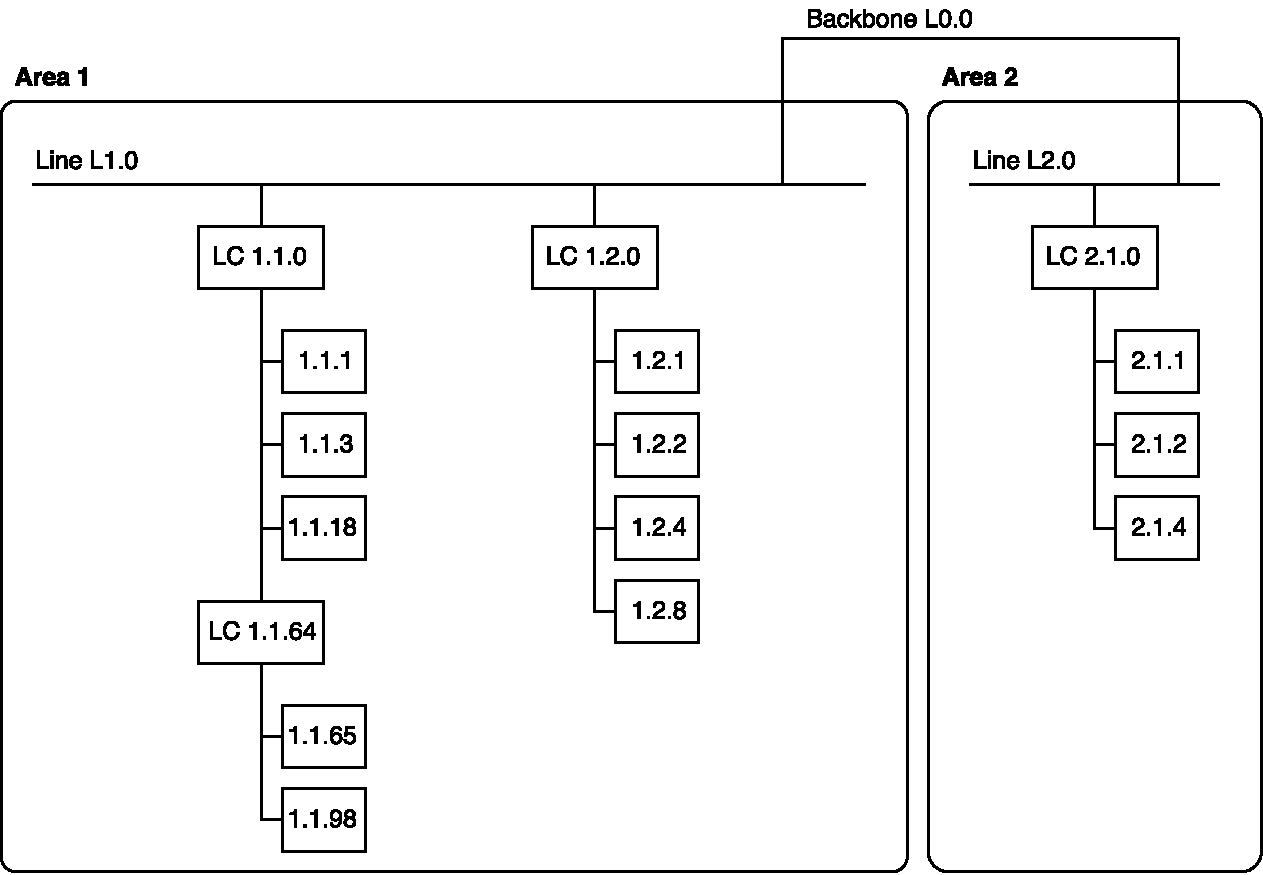
\includegraphics[width=\textwidth]{figures/100-knx-demo-topo.pdf}
	\caption[KNX network topology]{Exemplary logical topology of a \gls{knx} network with line couplers (LC) and normal devices.}
	\label{fig:background:knx:topo}
\end{figure}

The logical structure builds on top of the physical topology and is intended to remodel the functional structure of buildings in a logical tree topology. This tree topology is divided into three levels: areas, lines, and devices. Each device or node is assigned a physical address, defining area, line, and device number. (cf. Table~\ref{tab:background:bas:knx:topo:addr})
Each device is directly connected to a line, which can accommodate up to 256 devices, if supported by all devices on the line. Alternatively, up to 64 devices can be in one line segment before line repeater is required. (cf. Table~\ref{tab:background:bas:knx:topo:tpsegments})
Most \gls{knx} devices still follow the TP1-64 specification. Due to the high market fragmentation devices are often not mark in regards of supporting either TP1-64 or TP1-256, therefore it is still recommended to only use 64 devices within a line segment. \alert{sentence too long?} Thus, a full logical line is advised to be build using three line repeater. \parencite{Sokollik2017,Merz2009}

\begin{table}
	\aboverulesep=0ex
	\belowrulesep=0ex
	\renewcommand{\arraystretch}{1.2}
	
	\centering
	\begin{tabular}{|l|r|r|}
		\toprule
		& \textbf{TP1-64} & \textbf{TP1-256} \\\midrule
		maximum devices per segment & 64 & 256 \\
		maximum distance between 2 devices & 700m & 700m \\
		maximum length of a physical line & 1000m & 1000m \\
		\bottomrule
	\end{tabular}
	\caption[Segment properties for \knx.TP1-64 and \knx.TP1-256]{Segment properties for \knx.TP1-64 and \knx.TP1-256. cf. \textcite{Sokollik2017}}
	\label{tab:background:bas:knx:topo:tpsegments}
\end{table}

Usually a line coupler is installed as a line repeater. A line coupler is an active device to connect one logical level of the \gls{knx} network to another one, which can be one line segment to another line segment.
However, their original purpose is to separate the different levels of the logical \gls{knx} topology, explicitly to attach a line to the main line of an area or to attach a main line to the backbone. (cf. Figure~\ref{fig:background:knx:topo})
An area is formed by combining up to 16 lines: one main line and 15 sub-lines. All main lines are then connected to a backbone line, again via area couplers. \parencite{Sokollik2017}

As active devices line couplers are assigned addresses, and are able to filter traffic by addresses similar to \gls{ip} router. %usually with device number 0 in case it connects a line to backbone line.
Further couplers provide galvanic isolation to mitigate damages by high voltages, shorted circuits, etc. As a result multiple power supplies are required, basically one for each line segment.
An important feature to be aware of, when using line couplers, is that a \gls{knx} telegram can only be routed over six hops. This was introduced to prevent high network load in case of cyclic routing, comparable to the time to live in IP based networks. \parencite{Sokollik2017}

% KNX Address byte-field

\begin{table}[h]
	\aboverulesep=0ex
	\belowrulesep=0ex
	\renewcommand{\arraystretch}{1.2}
	
	\centering
	\begin{tabular}{|l|c|c|c|c|c|c|c|c|c|c|c|c|c|c|c|c|}
		\toprule
		Byte & \multicolumn{8}{c|}{1} & \multicolumn{8}{c|}{0} \\\midrule
		Bit & 7 & 6 & 5 & 4 & 3 & 2 & 1 & 0 & 7 & 6 & 5 & 4 & 3 & 2 & 1 & 0\\\midrule
		Physical Address & \multicolumn{4}{c|}{area} & \multicolumn{4}{c|}{line} & \multicolumn{8}{c|}{device}\\\midrule
		Group Address & \multicolumn{5}{c|}{main} & \multicolumn{3}{c|}{middle} & \multicolumn{8}{c|}{sub group}\\
		\bottomrule
	\end{tabular}
	\caption[Bit field for KNX addresses]{Bit field for \acs{knx} addresses. Only the most common used three-level group address is shown here. cf.~\textcite{Merz2009,Sokollik2017} }
	\label{tab:background:bas:knx:topo:addr}
\end{table}

Additional to the physical address each devices is assigned, devices may listen to group addresses.
\todo{describe layers/modes of group addresses?}
Whereby physical addresses are used to communicate with one specific device, which is common during installation, throughout normal operation mostly group addresses are used. As the name implies multiple devices may listen to such an address, allowing one light switch to turn on or off multiple lights for instance.

% ------------------------------------------------------------------------------	
\subsubsection{KNX Protocol}
\label{sec:background:bas:knx:proto}

\begin{comment}
		\begin{itemize}
		\item 3 types of telegrams \parencite{Hubner2009} \parencite{Merz2009}
			\subitem data - "sent in response to an individual action such as" \parencite{Merz2009} pressing a button (standard and extended \parencite{Hubner2009})
			\subitem acknowledge - "All devices (receivers) that belong to this group simultaneously confirm that they have received the data frame by returning an acknowledgment frame." \parencite{Merz2009}
			\subitem poll - "one device can query 1-Byte-Information from up to 15 other devices. Addressing is done via group addresses" \parencite{Hubner2009}
		\item Standard Data Telegram
			\subitem cf. Table~\ref{tab:background:bas:knx:proto:knx-standard}
		\item Extended Data Telegram
			\subitem cf. Table~\ref{tab:background:bas:knx:proto:knx-extended}
		\item Poll Telegram
			\subitem cf. Table~\ref{tab:background:bas:knx:proto:knx-poll}
		\item Acknowledge Telegram
			\subitem cf. Table~\ref{tab:background:bas:knx:proto:ack}
	\end{itemize}
\end{comment}

To communicate within a \gls{knx} network, devices send telegrams in their line. Due to the topology (cf. Section~\ref{sec:background:bas:knx:topo}) and technological nature of \gls{knx} these telegrams are always broadcasted within the respective line, only line couplers may narrow down the scope in which a specific telegram might be received. Telegrams are very comparable to packets in an IP network.

Within the \gls{knx} specification three types of telegrams are defined: Data Telegrams, Poll Telegrams, and Acknowledge Telegrams. (cf. Table~\ref{tab:background:bas:knx:proto:knx-standard},~\ref{tab:background:bas:knx:proto:ctrle},~\ref{tab:background:bas:knx:proto:knx-poll}, and~\ref{tab:background:bas:knx:proto:ack})
Each of which can be transmitted using on of four priorities, which are show in Table~\ref{tab:background:bas:knx:proto:prio}. Hereby it is to note, that a logical 0 is the dominant symbol. Consequently, the priority encoding is designed in a way, that lower priority telegrams are overruled by telegram with higher priority.
The bus devices detect these collisions and avoid them by following the \gls{csmaca} principle.

The telegram type is encoded in the first two bit of the \gls{ctrl} byte, which functions as a header of a \gls{knx} telegram. Next to the type it also contains a repeat flag, an acknowledge flag, and the priority. (see Figure~\ref{tab:background:bas:knx:proto:ctrl})

% KNX prio table

\begin{table}
	\aboverulesep=0ex
	\belowrulesep=0ex
	\renewcommand{\arraystretch}{1.2}
	\newcolumntype{Y}{>{\centering\arraybackslash}X}
	
	\centering
	\begin{tabularx}{0.7\textwidth}{|l|Y|Y|}
		\toprule
		Bit & 1 & 0 \\\midrule
		Function & \multicolumn{2}{c|}{Priority} \\\bottomrule
		\toprule
		System priority & 0 & 0 \\\midrule
		Alarm priority & 1 & 0 \\\midrule
		High priority & 0 & 1 \\\midrule
		Low priority & 1 & 1 \\\bottomrule
	\end{tabularx}
	\caption[\knx priority encoding]{\knx priority encoding. cf.~\textcite{Merz2009}}
	\label{tab:background:bas:knx:proto:prio}
\end{table}

%\subsubsection{Data Telegram}
\paragraph{Data Telegram}
\label{sec:background:bas:knx:proto:data}

The data telegram being utilised the most and used for transferring commands, state, and value changes, comes in two flavours.
The standard data telegram (cf. Table~\ref{tab:background:bas:knx:proto:knx-standard}) is able to transmit between 2 and 16 bytes per telegram. To transfer more data the extended data telegram (cf. Table~\ref{tab:background:bas:knx:proto:knx-extended}) can be utilised, which can transfer up to 255 bytes.
Both are sent in reaction of an direct interaction (e.g. light switch) or to send periodical sensor data (e.g. temperature). \parencite{Merz2009}
Once received and successfully processed, the recipient replies then with an acknowledge telegram. \parencite{Merz2009,Sokollik2017}

The extended data telegram introduces another header byte after \gls{ctrl}, the \gls{ctrle} header byte. It contains information otherwise encoded together with the payload length like the destination address type and the hop count, thus it allows the payload length to encoded as a full byte, ranging up to 255. (see Table~\ref{tab:background:bas:knx:proto:ctrle})

% KNX data telegram structure for standard and extended

\begin{table}
	\aboverulesep=0ex
	\belowrulesep=0ex
	\renewcommand{\arraystretch}{1.2}
	\newcolumntype{Y}{>{\centering\arraybackslash}X}
	
	\centering
	\begin{tabularx}{\textwidth}{|l|Y|Y|Y|Y|Y|Y|Y|Y|Y|Y|Y|Y|Y|Y|Y|Y|Y|Y|Y|Y|Y|Y|Y|Y|}
		\toprule
		Byte & \multicolumn{8}{c|}{0} & \multicolumn{8}{c|}{1} & \multicolumn{8}{c|}{2} \\\midrule
		Bit & & & & & & & & & & & & & & & & & & & & & & & & \\\midrule
		Function & \multicolumn{8}{c|}{CTRL} & \multicolumn{16}{c|}{Source Address} \\\bottomrule
		\toprule
		Byte & \multicolumn{8}{c|}{3} & \multicolumn{8}{c|}{4} & \multicolumn{8}{c|}{5} \\\midrule
		Bit & & & & & & & & & & & & & & & & & & & & & & & & \\\midrule
		Function & \multicolumn{16}{c|}{Destination Address} & \multicolumn{1}{c|}{\parbox[t][26pt][s]{0.2cm}{A T}} & \multicolumn{3}{c|}{Hops} & \multicolumn{4}{c|}{Length} \\\bottomrule
		\toprule
		Byte & \multicolumn{8}{c|}{6} & \multicolumn{8}{c|}{$7+n$} & \multicolumn{8}{c|}{$8+n$} \\\midrule
		Bit & & & & & & & & & & & & & & & & & & & & & & & & \\\midrule
		Function & \multicolumn{16}{c|}{Payload $n+1$ Bytes} & \multicolumn{8}{c|}{Parity} \\\bottomrule
	\end{tabularx}
	\caption[Standard \knx data telegram]{Standard \knx data telegram with $2$ to $16$ bytes of payload. Control Byte (CTRL) cf. Table~\ref{tab:background:bas:knx:proto:ctrl}, Source Address, Destination Address cf. Table~\ref{tab:background:bas:knx:topo:addr}, Address Type (AT), Hop Count (Hops), Payload Length (Length), Payload, and Parity.}
	\label{tab:background:bas:knx:proto:knx-standard}
\end{table}

\begin{table}
	\aboverulesep=0ex
	\belowrulesep=0ex
	\renewcommand{\arraystretch}{1.2}
	\newcolumntype{Y}{>{\centering\arraybackslash}X}
	
	\centering
	\begin{tabularx}{\textwidth}{|l|Y|Y|Y|Y|Y|Y|Y|Y|Y|Y|Y|Y|Y|Y|Y|Y|Y|Y|Y|Y|Y|Y|Y|Y|}
		\toprule
		Byte & \multicolumn{8}{c|}{0} & \multicolumn{8}{c|}{1} & \multicolumn{8}{c|}{2} \\\midrule
		Bit & & & & & & & & & & & & & & & & & & & & & & & & \\\midrule
		Function & \multicolumn{8}{c|}{CTRL} & \multicolumn{8}{c|}{CTRLE} & \multicolumn{8}{c|}{Source Address} \\\bottomrule
		\toprule
		Byte & \multicolumn{8}{c|}{3} & \multicolumn{8}{c|}{4} & \multicolumn{8}{c|}{5} \\\midrule
		Bit & & & & & & & & & & & & & & & & & & & & & & & & \\\midrule
		Function & \multicolumn{8}{c|}{Source Address} & \multicolumn{16}{c|}{Destination Address} \\\bottomrule
		\toprule
		Byte & \multicolumn{8}{c|}{6} & \multicolumn{8}{c|}{$7$} & \multicolumn{8}{c|}{$8+n$} \\\midrule
		Bit & & & & & & & & & & & & & & & & & & & & & & & & \\\midrule
		Function & \multicolumn{8}{c|}{Length} & \multicolumn{16}{c|}{Payload $n+1$ Bytes} \\\bottomrule
		\toprule
		Byte & \multicolumn{8}{c|}{$9+n$} & \multicolumn{16}{c|}{ } \\\cmidrule{1-9}
		Bit & & & & & & & & & \multicolumn{16}{c|}{ } \\\cmidrule{1-9}
		Function & \multicolumn{8}{c|}{Parity} & \multicolumn{16}{c|}{ } \\\bottomrule
	\end{tabularx}
	\caption[Extended \knx data telegram]{Extended \knx data telegram with $2$ to $255$ bytes of payload. Control Byte (CTRL) cf. Table~\ref{tab:background:bas:knx:proto:ctrl}, Extended Control Byte (CTRLE) cf. Table~\ref{tab:background:bas:knx:proto:ctrle}, Source Address, Destination Address cf. Table~\ref{tab:background:bas:knx:topo:addr}, Payload Length (Length), Payload, and Parity.}
	\label{tab:background:bas:knx:proto:knx-extended}
\end{table}
% KNX telegram CTRL byte

\begin{table}
	\aboverulesep=0ex
	\belowrulesep=0ex
	\renewcommand{\arraystretch}{1.2}
	\newcolumntype{Y}{>{\centering\arraybackslash}X}
	
	\centering
	\begin{tabularx}{\textwidth}{|l|Y|Y|Y|Y|Y|Y|Y|Y|}
		\toprule
		Byte & \multicolumn{8}{c|}{0} \\\midrule
		Bit & 7 & 6 & 5 & 4 & 3 & 2 & 1 & 0 \\\midrule
		Function & \multicolumn{2}{c|}{TT} & R & A & \multicolumn{2}{c|}{P} & \multicolumn{2}{c|}{reserved} \\\bottomrule \toprule
		Standard Data Telegram & 1 & 0 & R & 1 & \multicolumn{2}{c|}{P} & \multicolumn{2}{c|}{ } \\\midrule
		Extended Data Telegram & 0 & 0 & R & 1 & \multicolumn{2}{c|}{P} & \multicolumn{2}{c|}{ } \\\midrule
		Poll Telegram & 1 & 1 & 1 & 1 & 0 & 0 & \multicolumn{2}{c|}{ } \\\midrule
		Acknowledge Telegram & \multicolumn{2}{c|}{ } & 0 &0 & \multicolumn{2}{c|}{ } & \multicolumn{2}{c|}{ } \\\bottomrule
	\end{tabularx}
	\caption[\knx CTRL Byte]{\knx CTRL Byte. Telegram Type (TT), Repeat (R), Acknowledge (A), and Priority (P). cf. \textcite{Sokollik2017}}
	\label{tab:background:bas:knx:proto:ctrl}
\end{table}
% KNX CTRL-Extended control byte

\begin{table}[p]
	\aboverulesep=0ex
	\belowrulesep=0ex
	\renewcommand{\arraystretch}{1.2}
	\newcolumntype{Y}{>{\centering\arraybackslash}X}
	
	\centering
	\begin{tabularx}{0.7\textwidth}{|l|Y|Y|Y|Y|Y|Y|Y|Y|}
		\toprule
		Byte & \multicolumn{8}{c|}{0} \\\midrule
		Bit & 7 & 6 & 5 & 4 & 3 & 2 & 1 & 0 \\\midrule
		Function & AT & \multicolumn{3}{c|}{Hops} & \multicolumn{4}{c|}{EFF} \\\bottomrule
	\end{tabularx}
	\caption[\knx CTRLE Byte]{\knx CTRLE Byte. Address Type (AT), Hop Count, and Extended Frame Format (EFF). cf. \textcite{Sokollik2017}}
	\label{tab:background:bas:knx:proto:ctrle}
\end{table}

%\subsubsection{Acknowledge Telegram}
\paragraph{Acknowledge Telegram}
\label{sec:background:bas:knx:proto:ack}

The acknowledge telegram can indicate the correct reception (\code{ACK}, positive acknowledge), faulty reception (\code{NACK}, negative acknowledge), or that the receiving device is currently busy and is not able to process the telegram. (cf. Table~\ref{tab:background:bas:knx:proto:ack})
It consists of one byte and is sent by the recipient after waiting 13 bit times.
If the sender receives an positive acknowledge, the telegram was send successfully and no further action is required. However, if it detects an negative acknowledge or busy signal, the telegram is resend up to three times.
Supposed a busy signal occurred, the sender adds a waiting period before attempting to resend the telegram.
Given, the sender does not receives any form of acknowledge telegram within 13 bit times, it resends the telegram also up to three times.
In case the sender addressed the original telegram to multiple devices by using a group address as destination, the acknowledge frame is send simultaneously by all recipients. Due to the bus characteristic of being normally high (1), an negative acknowledge or busy signal overrules a positive acknowledge, since \code{BUSY} and \code{NACK} are encoded with low bits (0). \parencite{Merz2009,Sokollik2017}

\begin{table}[p]
	\aboverulesep=0ex
	\belowrulesep=0ex
	\renewcommand{\arraystretch}{1.2}
	\newcolumntype{Y}{>{\centering\arraybackslash}X}
	
	\centering
	\begin{tabularx}{0.7\textwidth}{|l|Y|Y|Y|Y|Y|Y|Y|Y|}
		\toprule
		Byte & \multicolumn{8}{c|}{0} \\\midrule
		Bit & 7 & 6 & 5 & 4 & 3 & 2 & 1 & 0 \\\bottomrule
		\toprule
		ACK  & 1 & 1 & 0 & 0 & 1 & 1 & 0 & 0 \\\midrule
		NACK & 0 & 0 & 0 & 0 & 1 & 1 & 0 & 0 \\\midrule
		BUSY & 1 & 1 & 0 & 0 & 0 & 0 & 0 & 0 \\\midrule
		NACK + BUSY & 0 & 0 & 0 & 0 & 0 & 0 & 0 & 0 \\\bottomrule
	\end{tabularx}
	\caption[KNX acknowledge telegram]{\gls{knx} short acknowledge telegram.}
	\label{tab:background:bas:knx:proto:ack}
\end{table}

%\subsubsection{Poll Telegram}
\paragraph{Poll Telegram}
\label{sec:background:bas:knx:proto:poll}

The poll telegram allows to poll one byte of data from up to 15 devices, however, it is seldom used in \gls{knx} networks. It consists of a poll data request frame (cf. Table~\ref{tab:background:bas:knx:proto:knx-poll}) and a poll data response frame. Former starts the poll telegram and sets the group address to query, also it defines how many bytes to receive.
The poll data response consists of each device sending one byte on the bus without starting a new telegram. The responding devices are doing so in a prior configured time slot. \parencite{Hubner2009,DIN_EN_50090-5-2}

\begin{table}[p]
	\aboverulesep=0ex
	\belowrulesep=0ex
	\renewcommand{\arraystretch}{1.2}
	\newcolumntype{Y}{>{\centering\arraybackslash}X}
	
	\centering
	\begin{tabularx}{\textwidth}{|l|Y|Y|Y|Y|Y|Y|Y|Y|Y|Y|Y|Y|Y|Y|Y|Y|Y|Y|Y|Y|Y|Y|Y|Y|}
		\toprule
		Byte & \multicolumn{8}{c|}{0} & \multicolumn{8}{c|}{1} & \multicolumn{8}{c|}{2} \\\midrule
		Bit & & & & & & & & & & & & & & & & & & & & & & & & \\\midrule
		Function & \multicolumn{8}{c|}{CTRL} & \multicolumn{16}{c|}{Source Address} \\\bottomrule
		\toprule
		Byte & \multicolumn{8}{c|}{3} & \multicolumn{8}{c|}{4} & \multicolumn{8}{c|}{5} \\\midrule
		Bit & & & & & & & & & & & & & & & & & & & & & & & & \\\midrule
		Function & \multicolumn{16}{c|}{Destination Address} & \multicolumn{4}{c|}{ } & \multicolumn{4}{c|}{poll data} \\\bottomrule
		\toprule
		Byte & \multicolumn{8}{c|}{6} & \multicolumn{16}{c|}{ } \\\cmidrule{1-9}
		Bit & & & & & & & & & \multicolumn{16}{c|}{ } \\\cmidrule{1-9}
		Function & \multicolumn{8}{c|}{Parity} & \multicolumn{16}{c|}{ } \\\bottomrule
	\end{tabularx}
	\caption[KNX poll telegram]{\gls{knx} poll telegram. Control Byte (CTRL) cf. Table~\ref{tab:background:bas:knx:proto:ctrl}, Source Address, Destination Address cf. Table~\ref{tab:background:bas:knx:topo:addr}, expected length of poll data (poll data), and Parity.}
	\label{tab:background:bas:knx:proto:knx-poll}
\end{table}

\subsubsection{KNX Communication}
\label{sec:background:bas:knx:communication}

\begin{comment}
		\begin{itemize}
		\item application layer described in \textcite{DIN_EN_50090-4-1}
		\item communication modes \parencite{DIN_EN_50090-4-1}
			\subitem point-to-multipoint, connection-less (multicast)
			\subitem point-to-domain, connection-less (broadcast)
			\subitem point-to-all-points, connection-less (system broadcast)
			\subitem point-to-point, connection-less
			\subitem point-to-point, connection-oriented
		\item APCI describes operation on application layer
		\item Response need to match the Request APCI type and must be send on the corresponding communication mode allowed for this packet. cf. \textcite[][page 9--10]{DIN_EN_50090-4-1}
	\end{itemize}
\end{comment}

Apart from the basic \gls{knx} protocol (cf. Section~\ref{sec:background:bas:knx:proto}), which is comparable to the data link layer in the \gls{osi} model, the \textcite{DIN_EN_50090-4-1} describes two layers on top: a transport layer and an application layer.
However, it is to note, that even when official \gls{knx} specification draws parallels to the \gls{osi} model, a direct comparison to the \gls{osi} model as seen in \gls{ip} networks is difficult, due to the reduced complexity of the protocol stack in \gls{knx}.

The transport layer defines multiple transport layer services, which are encoded in the \gls{tpci} (cf. Table~\ref{tab:background:bas:knx:comm:tpci-apci}) and can be clustered into five categories or modes:

\begin{enumerate}
	\item point-to-multipoint, connection-less (multicast)
	\item point-to-domain, connection-less (broadcast)
	\item point-to-all-points, connection-less (system broadcast)
	\item point-to-point, connection-less
	\item point-to-point, connection-oriented
\end{enumerate}
\parencite[p.~30]{DIN_EN_50090-4-2}

Depending on the category, multiple telegrams might be send in order to establish a connection, e.g. point-to-point, connection oriented.
Further, these communication modes are used by the 44 different application layer services described in \textcite{DIN_EN_50090-4-1}.
These application layer services can be used to access and set device states, encoded in \glspl{dpt}, or to configure the device.
Each response needs to match the requests \gls{apci} type and must be send on with the corresponding communication mode allowed for this telegram. \parencite[pp.~9--10]{DIN_EN_50090-4-1}

\glspl{dpt}, in turn, define the structure of the data, which is transported using the application layer services.
They are defined to consist of a combination of a data type and a dimension. Whereby the former is required to specify format and encoding. The later, however, defines range and unit.
It was decided not to specify data types and dimensions separately to reduce abstract naming and confusion.
Therefore any \gls{dpt} declares a single combination of format, encoding, range, and unit. \parencite[p.~38]{DIN_EN_50090-3-3}

Each \gls{dpt} is identified by an 16 bit main number and an 16 bit sub-number, separated by a dot. The main number describes the format and encoding and consequently the sub-number describes range and unit. As a result, \glspl{dpt} with the same main number share the format and encoding.

\begin{table}
	\aboverulesep=0ex
	\belowrulesep=0ex
	\renewcommand{\arraystretch}{1.2}
	\newcolumntype{Y}{>{\centering\arraybackslash}X}
	
	\centering
	\begin{tabularx}{\textwidth}{|l|Y|Y|Y|Y|Y|Y|Y|Y|Y|Y|Y|Y|Y|Y|Y|Y|}
		\toprule
		Byte & \multicolumn{8}{c|}{6} & \multicolumn{8}{c|}{7} \\\midrule
		Bit & & & & & & & & & & & & & & & & \\\midrule
		\multirow{2}{*}{Function} & \multicolumn{6}{c|}{TPCI} & \multicolumn{10}{c|}{APCI} \\\cmidrule{2-7}
		 & DC & No & \multicolumn{4}{c|}{Seq. Number} & \multicolumn{10}{c|}{} \\\bottomrule
	\end{tabularx}

	\caption[KNX TPCI/APCI structure in a standard data telegram]{\gls{knx} \acrshort{tpci}/\acrshort{apci} structure in a standard data telegram. Data/Control flag (DC), Numbered/Unnumbered flag (No), Sequence Number (Seq. Number).}
	\label{tab:background:bas:knx:comm:tpci-apci}
\end{table}
	
\subsubsection{KNX Management Procedures}
\label{sec:background:bas:knx:management}

\begin{comment}
	\begin{itemize}
		\item "describe the device independent management procedures" \parencite{DIN_EN_50090-7-1}
		\item "shall be used to configure the network, and to get the information about the configuration of the network and connected devices" \parencite{DIN_EN_50090-7-1}
		\item " no knowledge of the single devices is required. They will work with every device connected to the network" \parencite{DIN_EN_50090-7-1}
		\item "shall be based on the use of the dedicated application layer services which are specified in EN 50090-4-1 \parencite{DIN_EN_50090-4-1} for this purpose" \parencite{DIN_EN_50090-7-1}
	\end{itemize}
\end{comment}

To ensure maximum compatibility among \gls{knx} devices of different vendors, it is not only sufficient these devices implement the same protocol stack (cf. Section~\ref{sec:background:bas:knx:proto}) and use the same communication services (cf. Section~\ref{sec:background:bas:knx:communication}).
Moreover, it is also required that they share a common set of management and configuration services.
This is especially true in an environment like \gls{knx}, where devices need to be fully interchangeable and need to be configurable by a common tool used by electricians.

Therefore, the \gls{knx-assoc} specified two sets of management procedure.
For these procedures dedicated application layer services were defined in \textcite{DIN_EN_50090-4-1}. (cf. Section~\ref{sec:background:bas:knx:communication})
The first, being called network management procedures, are device independent, which do not require any knowledge or insight of the devices and will work across all vendors and device types. \parencite[pp.~11~ff.]{DIN_EN_50090-7-1}
They mainly provide routines to configure addresses, read serial numbers, get functions, or to find all devices in programming mode.

Secondly, there are device management procedures, which require in depth knowledge of the devices. \parencite[pp.~30~ff.]{DIN_EN_50090-7-1}
These are used to i.e. configure devices, restart them, and verify the configuration.

\subsubsection{Security in KNX}
\label{sec:background:bas:knx:security}

\begin{comment}
	\begin{itemize}
		\item copulers allow filtering 
			\subitem "This means that data frames transmitted by a sender are only forwarded to recipients that are not on the sender’s line." \parencite{Merz2009}
			\subitem "The filter function only forwards data frames to where they are needed. This reduces the overall amount of data frame traffic and keeps the data traffic on one line separate from the data traffic on another line, allowing data to be transferred on several lines simultaneously." \parencite{Merz2009}
		\item main group 14 and 15 should not be used \parencite{Hubner2009}
			\subitem can not be filtered due to limited space for filter tables in couplers \parencite{Hubner2009}
			
		\item cf DIN50090-3-4 page 13 (secure application layer) \parencite{DIN_EN_50090-3-4}
	\end{itemize}
\end{comment}

With \gls{knx} being so widely used, it is also deployed in security sensitive areas like access control\footnote{\url{http://search-ext.abb.com/library/Download.aspx?DocumentID=2CDC500074M0201&LanguageCode=en&DocumentPartId=&Action=Launch}}, ventilation, or fire alarms\footnote{\url{https://www.knx.org/media/docs/downloads/Marketing/Flyers/KNX-Solutions/KNX-Solutions_en.pdf}}.
As a consequence it is only sensible to consider not only the operational safety, but also the information security of \gls{knx} networks. Meaning, it should not only be assured, that the network is operational at any time, but it needs to be protected against malicious usage or intrusion.
This is especially vital, if gateways to \gls{ip} networks exists as these are easily exposed to the internet.

By design \gls{knx} introduces a zone concept by distinguishing between lines and areas.
This offers the possibility to limit a potential attack to just one line, because the traffic between lines is filtered by line couplers.
This filter function ensures, that only traffic concerning devices in other lines is routed to the main or backbone line.

However, filtering traffic comes with certain limitations. For instance the line couplers need be configured properly, which can be done automatically by the installation and configuration Software \gls{ets}. \parencite{Merz2009}
Further, to ensure proper filtering the main groups 14 and 15 must not be used, since they cannot be filtered, due to limited space for filter tables in couplers. \parencite{Hubner2009}
Moreover, traffic within the affected line can still be red and manipulated by an attacker, as well as device can be reconfigured or attacked.

Another possibility to secure a \gls{knx} network is to enable \gls{s-al}, as defined in \textcite{DIN_EN_50090-3-4}. \Gls{s-al} is an extension of the \gls{knx} specification defining an encrypted application layer (cf. Section~\ref{sec:background:bas:knx:communication}) for multicast and point-to-point communication, which can be used next to normal unencrypted traffic.
As encryption standard \textcite{DIN_EN_50090-3-4} defines \acs{aes}-128 in \gls{ctr} or \gls{ccm} mode.
Later also functions as authentication. \todo{ensure short formes are used, at least for AES}

Nonetheless it is to note, that \textcite{DIN_EN_50090-3-4} is merely a draft at the point of June 2017.
Therefore, it is not to expect, that available \gls{knx} devices with this capability will be on the market any time soon. This may also be caused by the relatively high life time of devices which are installed permanently in buildings, which have an expected lifetime of up to 40 years.


% ------------------------------------------------------------------------------
%\section{\lonworks}

%\section{\bacnet}
	
	%\chapter{Network Analysis and Flow Monitoring}
	\section{Network Analysis and Flow Monitoring}
	% background about netflow
	\label{sec:background:network}
	% !TeX spellcheck = en_GB

\todo{general introductory sentence about network mon}

\subsection{Intrusion Detection Systems (IDS)}
\label{sec:background:network:ids}

\begin{comment}
		\begin{itemize}
		\item \enquote{A good network intrusion detection system (IDS) can have an enormous positive impact on the overall security of your oragnization} \parencite{Northcutt2005}
		\item \enquote{By detecting malicious activity, network intrusion detection enables you to identify and react to threats against your environment, as well as threasts that your hosts might be directing at hosts on other networks.} \parencite[p. 201]{Northcutt2005}
		\item \enquote{Without intrusion detection, you may never know about an attack that doesn't damage your host, but simply extracts information[...]. Without intrusion detection, you will be unaware of these events until it's much too late.} \parencite[p. 202]{Northcutt2005}
		\item Not only identifies attacks, but also reveals attack attempts and probing \parencite[p. 202]{Northcutt2005}
		\item 
	\end{itemize}
\end{comment}

Good network security consists of many parts, covering a huge variety of methods and functions. \hint{This sounds weird and artificial.}
As one of these parts \enquote{a good \gls{ids} can have an enormous positive impact on the overall security [...]}. \parencite{Northcutt2005}
The basic idea is to monitor the network traffic passing by sensors and therefore be able to detect malicious activities.
This allows the \gls{ids} to detect and identify threasts against the own environment or theats ones own hosts impose to other environments, due to an infection with malware.
Without intrusion detection one might never detect attacks, that do not influence normal operations but for instance extract information.

Further, \gls{ids} may also identify attack attempts and probing, allowing to further harder the environment and take precautions.

Nowadays \glspl{ids} are a commonly deployed in \gls{ip} networks. There are different kinds of \glspl{ids}, which can be discriminated by working principle. The following section is giving an overview of the most common technologies. \parencite[cf.][pp.~201-202]{Northcutt2005}

\subsubsection{Signature-based Intrusion Detection Systems (SIDS)}
\label{sec:background:network:ids:sig}

\begin{comment}
	\begin{itemize}
		\item \enquote{[...] IDS signature is a pattern you are looking for in traffic.} \parencite{Northcutt2005}
		\item \enquote{When a signature for an attack matches observed traffic, an alert is generated, or the event is otherwise recorded.} \parencite{Northcutt2005}
		\item \enquote{Many signatures are protocol or application specific;} \parencite{Northcutt2005}
		\item requires to update a curated set of signatures regularly \parencite{Northcutt2005}
		\item \enquote{Signature development is always a balancing act. A specific signature might be extremely accurate in identifying a particular attack [...] [but] If an attacker slightly modifies the attack, the signature might not be able to identify it at all.} \parencite{Northcutt2005}
			\subitem precision/recall balance
		\item \enquote{Every intrusion detection system generates false positives.} \parencite[p.~205]{Northcutt2005}
		\item \enquote{By selecting a solid IDS product and tuning your sensors, you can reduce false positives, but you can't completely eliminate them.} \parencite[p.~205]{Northcutt2005}
		\item \enquote{[...], but each false negative is a legitimate attack or incident that IDS failed to notice.} \parencite[p.~206]{Northcutt2005}
		\item \enquote{Besides false positives, you might also have alerts that address legitimate problems that you simply don't care about.} (Unwanted Alerts) \parencite[p.~206]{Northcutt2005}
		\item 
	\end{itemize} 
\end{comment}

One of the more traditional \gls{ids} principles are signature based systems.
They work by comparing patterns (signatures) of malicious traffic to the observed traffic. When a pattern matches an alert is raised.
This requires many protocol and application specific signatures, which are difficult to create and maintain, since a good balance between being too generic and being too specific needs to be found.

A signature which is too generic, may cause many false positives. This might lead to an elimination of any positive effect of the \gls{ids}, since real alerts become impossible to spot among the false positives.
In contrast, however, a signature which is too specific might suffer from a too narrow scope. Meaning, that it might be really precise in classifying one particular attack, but fails to do so if an attacker just slightly modifies it.

As a result, a valuable \gls{ids} solution is characterised by an balanced precision/recall ratio. This can be archived by using a good signature database and fine tuning the sensors.
However, it is to note, that every \gls{ids} will produce false positives. This derives out of the consideration, that each false negative is an legitimate attack, which was not detected. Therefore a slight tendency to (over) sensitivity is sensible.

Other than false positives, there might be legitimate alerts that are of no interest. These unwanted alerts should be blocked, to not numb \alert{(is this the right word here?)} the system administrator. \parencite[cf.][pp.~205-206]{Northcutt2005}
	
\subsubsection{Anomaly-based Intrusion Detection Systems (ABIDS)}
\label{sec:background:network:ids:anomaly}
	
\begin{comment}
	\begin{itemize}
		\item \enquote{establishing baselines of normal network activity over a period of time, then detecting significant deviations from the baseline.} \parencite[p. 203]{Northcutt2005}
		\item \enquote{[...] later, if the IDS sensor sees a high volume of traffic involving a previously unused service on a host, this could indicate a distributed denial of service (DDoS) attack against the host or a compromised host providing a new service.} \parencite{Northcutt2005}
		\item \enquote{[...] drawback of this type of anomaly detection is that the baseline needs to be updated constantly to reflect authorized changes[...]} \parencite{Northcutt2005}
		\item \enquote{If the baseline can be kept current, or if the environment is quite static and the baseline changes rarely, anomaly detection can be extremely effective at identifying certain types of attacks [...]} \parencite{Northcutt2005}
		\item \textbf{\enquote{Unfortunately, this type of anomaly detection cannot identify most other types of attacks, so it is best used to complement other IDS technologies.}} \parencite{Northcutt2005}
		\item \enquote{[...] can [...] identifying certain previously unknown instances of attacks [...]} \parencite{Northcutt2005}
		\item \enquote{cannot determine the intent of an attack} \parencite{Northcutt2005}
	\end{itemize}
\end{comment}

Another major technology used in \glspl{ids} is anomaly detection. (cf. Section~\ref{sec:background:network:novelty})
Unlike signature based methods (cf. Section~\ref{sec:background:network:ids:sig}) it does not require an predefined set of rules, rather deploying anomaly detection it is able to auto-generate rules specific for the monitored network and then perform whitelisting using these rules.

This is archived by having a so called training phase before deploying the \gls{ids}. During the training phase a baseline model is established using the normal network activity over period of time. It is to note, that this period should be long enough to cover normally recurring usage cycles, e.g. day-time/night-time, weekday/weekends, etc.

After an successful training phase the \gls{ids} uses the generated baseline model to compare bypassing traffic against it.
If it detects a significant deviation from it, an alert is raise as it indicates unusual network activities.
For instance, if an internal host in an \gls{ip} network, produces suddenly a lot of outbound traffic, which was not the case before, it might indicate an infection on this host.

This example illustrates 2 primary drawbacks of purely anomaly-based \glspl{ids}: 
First, the system can not identify which kind of attack it detects, it merely identifies an anomaly. To identify the intention of the attack it would need to be combined with a rule system or signature-based approach.

Second, the increased outbound traffic in the example could have been generated by a new legitimate software, i.e. a website crawler.
Consequently, strictly separated training and operational phases lead to poor adaption of the \gls{ids} to a changing environment.
This could be mitigated by updating the baseline model during normal operation, so t accommodates for changes.
However, by continuing the training phase, attacker might be able to reprogram the baseline in their favour by injecting malicious packets very rarely at the beginning, but then increase the amount steadily.
By doing so the relative deviation from the continuing trained baseline model stays relatively low and will therefore not trigger an alert.
This means, the decision if the baseline model should be trained continuously has to be made under careful consideration of the nature of the network to be monitored.

All in all, anomaly-based \glspl{ids} are ideal to identify prior unknown threats and attacks in relatively stable environments. However, it might also identify (legitimate) changes in the environment as anomaly. Additionally it might be unable to detect attacks which mimic regular behaviour and only deviate slightly from legitimate traffic.
As a result, anomaly-based \glspl{ids} should be combined with other \gls{ids} technologies, when used to protect production systems.
\parencite[cf.][pp.~203-204]{Northcutt2005} \todo{check pages}
	
\subsubsection{State-based Intrusion Detection Systems\hint{??}}
\label{sec:background:network:ids:state}

\begin{itemize}
	\item cf. \textcite{Whitman2009} page 306 
\end{itemize}

% ------------------------------------------------------------------------------
\subsection{Flow Monitoring}
\label{sec:background:network:netflow}

\begin{comment}
	\begin{itemize}
		\item active
			\begin{itemize}
				\item inject additional traffic to measure things \parencite{Hofstede2014}
				\item e.g. ping, traceroute
			\end{itemize}
		\item passive
			\begin{itemize}
				\item "observe existing traffic as it passes by" \parencite{Hofstede2014}
				\item e.g. packet capture "This method generally provides most insight into the network traffic, as complete packets can be captured and further analyzed. However, in high-speed networks with line rates of up to 100 Gbps, packet capture requires expensive hardware and substantial infrastructure for storage and analysis." \parencite{Hofstede2014}
				\item "Another passive network monitoring approach that is more scalable for use in high-speed networks is flow export, in which packets are aggregated into flows and exported for storage and analysis." \parencite{Hofstede2014}
				\item  "a set of IP packets passing an observation point in the network during a certain time interval, such that all packets belonging to a particular flow have a set of common properties." \parencite{Claise2013}
				
			\end{itemize}
	\end{itemize}
\end{comment}

Following the idea of network monitoring with \glspl{ids}, multiple method are being used. They can be roughly classified into active and passive. 
Active approaches work by injecting additional traffic into the network to obtain certain measurements, like ping or traceroute.
Passive techniques, on the contrary, only observe existing traffic passing by a measurement point and derive measurements from it. The most simple and straight forward passive approach would be packet capturing. Also it provides the most insights into bypassing traffic, since in-depth analysis are possible. However, a full packet capture raises problem within high-speed networks or if network bandwidth is highly limited, like it is in field bus networks. This is especially problematic if information are required to be analysed by an central authority to obtain world-view. The problems arising here include high storage consumption, excessive infrastructure requirements, and unnecessary high utilisation of network bandwidth. \todo{relevant in already highly utilised networks, etc.}
\parencite[cf.][]{Hofstede2014}
Especially the additional high network utilisation is of notable concern in field bus networks used in \glspl{bas}. Effectively doubling the traffic in the sub-lines, as well as routing the monitoring traffic to central place would not only occupy a good portion of free bus capacity, but would also render network separation (cf. Section~\ref{sec:background:bas:knx:security}) useless. Consequently, soften the security in the network and possibly decreasing the responsiveness of commands dramatically.

A another predominantly used passive approach is flow monitoring, which focusses on analysing flows within a network rather than analysing a full packet dump. Therefore archiving a significant data reduction and consequently requiring only a fraction of the bandwidth, while also keeping principles like network separation in tact, since only aggregated statistical data is transferred.
A flow is defined by \textcite{Claise2013} as \enquote{a set of IP packets passing an observation point in the network during a certain time interval, such that all packets belonging to a particular flow have a set of common properties.}
Mentioned common properties most commonly include various header fields, like port, source- and destination address, but also the used application layer protocol or metadata derived from the packet content.
It is widely used for \enquote{security analysis, capacity planning, accounting, and profiling, among others.} \parencite{Hofstede2014}
Common protocols used for flow monitoring are \gls{netflow} \parencite{Claise2004} and \gls{ipfix} \parencite{Claise2013}.

\todo{not predominantly used for security, but network congestion avoidance/mitigate.}

\begin{figure}
	\centering
	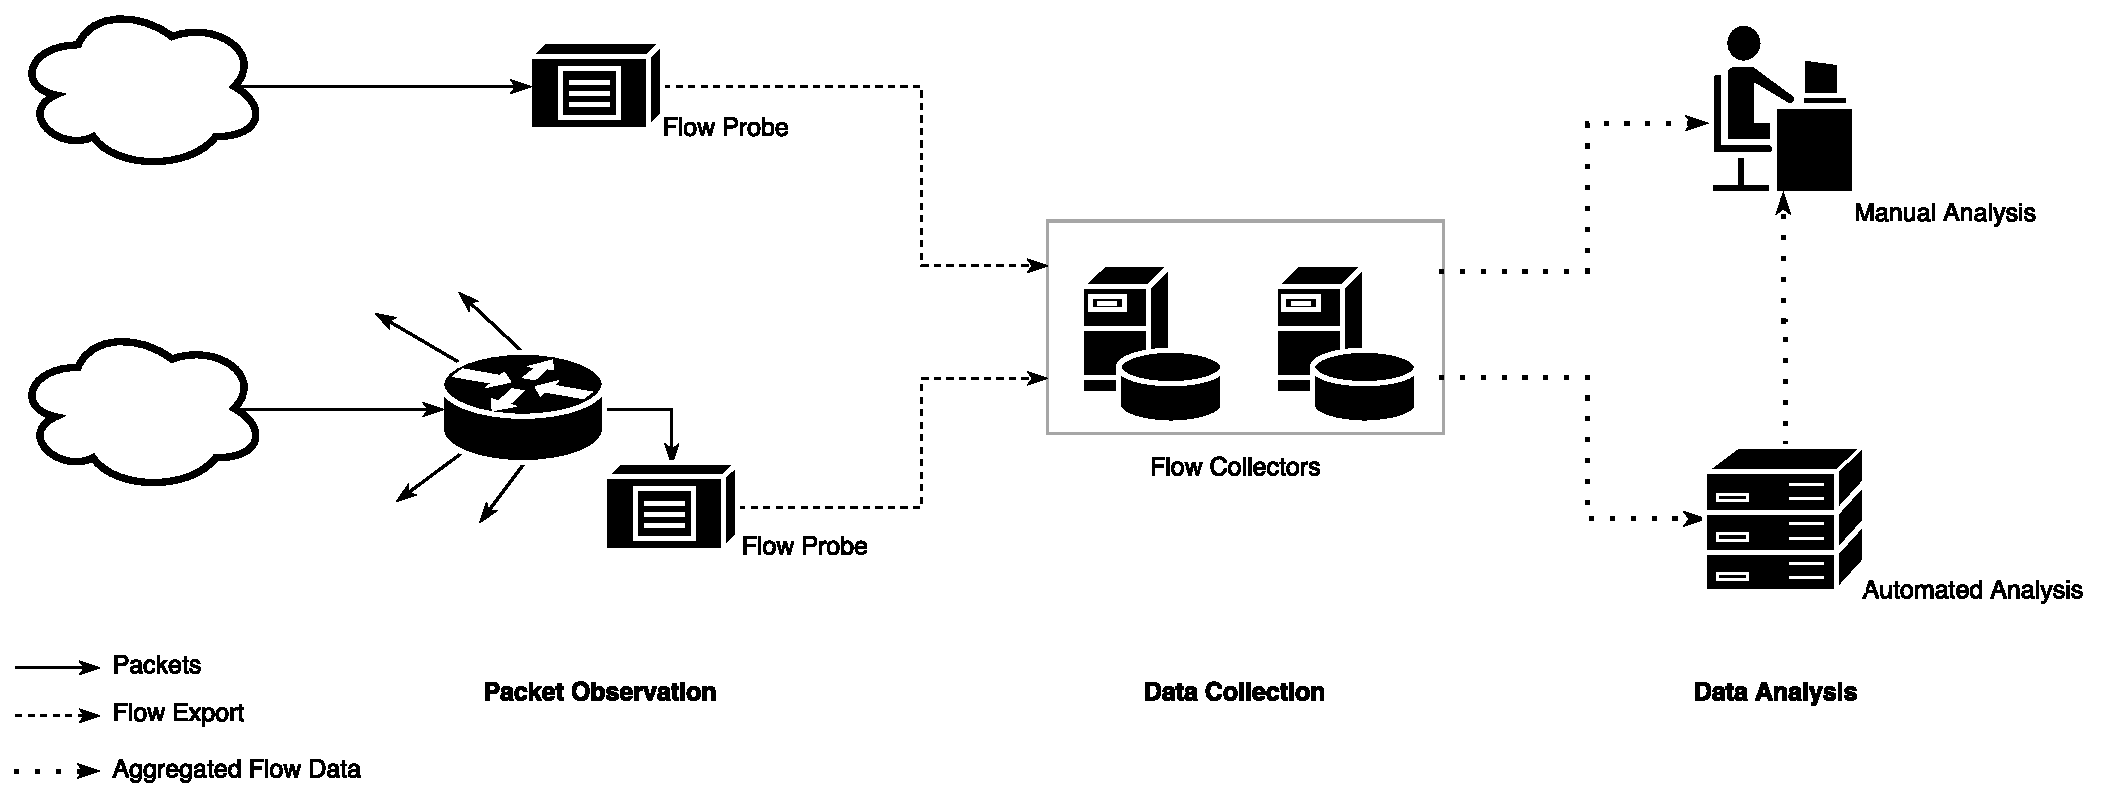
\includegraphics[width=\textwidth]{figures/200-netflow-architecture.pdf}
	\caption[Simplified flow monitoring system architecture]{Simplified flow monitoring system architecture. \parencite[cf.][]{Hofstede2014} \todo{adjust font size}}
	\label{fig:background:network:netflow:architecture}
\end{figure}

Typical flow monitoring architectures can be roughly separated into 3 stages. (cf. Figure~\ref{fig:background:network:netflow:architecture})
The first one, being Packet Observation and Flow Export, will observe bypassing traffic. Further the observed traffic is aggregated into flows, using common properties as selectors. (cf. above\alert{???}) After a flow is terminated, either by closing the underlying connection or by timeout, a record of it is exported and send of to the Flow Collector.
This stage could be implemented by a stand-alone device or within an appliance like a router with flow export capability. \parencite[cf.][]{Hofstede2014}

The exported flow are then receive by the Data Collector, which main task are storage and processing.
Exported flows contain \enquote{information about a specific flow that was observed at an observation point} \parencite{Claise2013}, which may include characteristic properties like \gls{ip} addresses and port number, as well as measured properties like packet count or overall flow size in bytes. \parencite[cf.][]{Hofstede2014}
In scope of \glspl{bas}, like \gls{knx}, characteristic properties could include source and destination address, and \gls{apci}. Hop count, payload length, and \gls{tpci} would then be used as measured properties.

Finally the last stage is concerned with the data analysis. This can be done in a manual, exploratory way, which is often the case in research projects. In more production oriented setups the analysis is often automated and integrated into the Data Collector.
The data analysis commonly includes functions like traffic profiling, correlation, anomaly and intrusion detection (cf. Section~\ref{sec:background:network:ids}), and classification and characterisation. \parencite[cf.][]{Hofstede2014}
In this work mainly anomaly and intrusion detection is of interest.

% ------------------------------------------------------------------------------
\section{Anomaly, Outlier, and Novelty Detection}
\label{sec:background:network:novelty}

The analysis of flows or general network traffic as describes in Section~\ref{sec:background:network:ids:anomaly}~and referenced in Section~\ref{sec:background:network:netflow}, relies on algorithm and techniques to detect data points which deviate from the normal expected behaviour. These algorithms and techniques can be found \alert{(better phrasing)} under the term Anomaly, Outlier, or Novelty Detection.
The aim of this section is to provide a classification of these algorithms with benefits and drawbacks.
Further, an overview of the working principle is provided for a small selection of them.

% ------------------------------------------------------------------------------
\subsection[Classification of Anomaly, Outlier, and Novelty Detection]{Classification of Anomaly, Outlier, and Novelty Detection Approaches}
\label{sec:background:network:novelty:class}

\begin{comment}
	\begin{itemize}
		\item cf. \textcite{Hodge2004}
		\item Type 1: "Determine the outliers with no prior knowledge of the data" \parencite{Hodge2004}
			\subitem "unsupervised clustering" \parencite{Hodge2004}
			\subitem "assumes that errors or faults are separated from the ‘normal’ data and will thus appear as outliers" \parencite{Hodge2004}
			\subitem " predominantly retrospective and is analogous to a batch-processing system" \parencite{Hodge2004} - Requires a bunch of data to begin with
			\subitem " requires that all data be available before processing" \parencite{Hodge2004}
			\subitem "data is static" \parencite{Hodge2004}
			\subitem "two sub-techniques" \parencite{Hodge2004}
			\subitem -> "outlier diagnostic approach highlights the potential outlying points" \parencite{Hodge2004} and "prune the outliers and fit their system model to the remaining data until no more outliers are detected" \parencite{Hodge2004}
			\subitem -> "accommodation that incorporates the outliers into the distribution model generated and employs a robust classification method" \parencite{Hodge2004} which "can withstand outliers in the data and generally induce a boundary of normality around the majority of the data" \parencite{Hodge2004}
			\subitem "Non-robust methods are best suited when there are only a few outliers in the data set" \parencite{Hodge2004}
			\subitem "a robust method must be used if there are a large number of outliers to prevent this distortion" \parencite{Hodge2004}
		\item Type 2: "Model both normality and abnormality." \parencite{Hodge2004}
			\subitem "supervised classification" \parencite{Hodge2004}
			\subitem "requires pre-labelled data" \parencite{Hodge2004}
			\subitem "The entire area outside the normal class represents the outlier class" \parencite{Hodge2004}
			\subitem "best suited to static data" \parencite{Hodge2004} "classification needs to be rebuilt from first principles if the data distribution shifts" \parencite{Hodge2004}
			\subitem "can be used for on-line classification" \parencite{Hodge2004} learning while new samples are classified
			\subitem "require a good spread of both normal and abnormal data" \parencite{Hodge2004}
			\subitem "classification is limited to a ‘known’ distribution" \parencite{Hodge2004}
			\subitem "cannot always handle outliers from unexpected regions" \parencite{Hodge2004}
		\item Type 3: "Model only normality [...]" \parencite{Hodge2004}
			\subitem "novelty detection" \parencite{Hodge2004} " semi-supervised recognition or detection task" \parencite{Hodge2004}
			\subitem "needs pre-classified data but only learns data marked normal" \parencite{Hodge2004}
			\subitem "suitable for static or dynamic data" \parencite{Hodge2004}
			\subitem "can learn the model incrementally as new data arrives" \parencite{Hodge2004}
			\subitem "aims to define a boundary of normality" \parencite{Hodge2004}
			\subitem "requires the full gamut of normality to be available for training to permit generalisation" \parencite{Hodge2004} but "requires no abnormal data" \parencite{Hodge2004}
			\subitem this is good, because "Abnormal data is often difficult to obtain or expensive in many fault detection domains [...]" \parencite{Hodge2004}
			\subitem "as long as the new fraud lies outside the boundary of normality then the system will be correctly detect the fraud" \parencite{Hodge2004}
	\end{itemize}
\end{comment}

Anomaly, Outlier, or Novelty Detection describes a class of algorithms to detect data points which deviate from the expected normal behaviour.
Or as defined by \textcite{Grubbs1969}, \enquote{an outlying observation, or outlier, is one that appears to deviate markedly from other members of the sample in which it occurs.}
In the following this definition will be used as an understanding for outliers, which is exchangeable for anomaly or novelty. \alert{(think about this!)}

The general class of algorithms for Anomaly, Outlier, and Novelty Detection can be divided into 3 sub-classes, based on which kind of data the algorithms require to be trained\alert{~and executed}.
The first sub-class describes algorithms, which are able detect outliers without prior knowledge of the data, also known as unsupervised clustering.
This means, the data points in a training set are not require to be labelled as \emph{normal} or \emph{outlier}, which is archived by relying on the assumption, that non-normal data is separated from normal data, thus appearing as outlier.
Accordingly, a substantial amount of data is required to begin with, since these kind of algorithms word \enquote{predominantly retrospective} \parencite{Hodge2004}.
Thus requiring (all) data to be available before processing and assuming it to be static.
Within this technique, 2 approaches  are used for training the model. 
The first identifies potential outliers and then continues to prune them from the original data set and fit the model to the remaining data points. This is iterated until no more outliers are detected. This non-robust method is well suited when only a few outliers are in the data set.
The second approach, however, accommodates the outliers into the distribution model and then applies a robust classification method. This is a better suited for data sets with higher numbers of outliers, since a robust classification method can withstand outliers in the data set by inducing boundaries of normality around large portions of the data. \parencite[cf.][]{Hodge2004}

The second sub-class within Outlier Detection techniques works by modelling both, normality and outliers, it is also known as supervised classification.
Therefore it requires pre-labelled data in the training phase, labelled as \emph{normal} or \emph{outlier}. Since both are used to build the model, a good spread of \emph{normal} and \emph{outlying} data is required, which also limits the classification to the known distribution of such.
As a result the whole classification model needs to be rebuild from ground up, as soon as the distribution shifts.
However, a major benefit of this method is, that it is allows for training the model while new data points are being classified, which is also known as on-line classification. \parencite[cf.][]{Hodge2004}

The third and last sub-class in Outlier Detection techniques models only normality. These techniques are often described as novelty detection or semi-supervised recognition.
It requires also pre-labelled data, but compared to the second type it only works with \emph{normal} labelled data points. Consequently the full gamut of normality is required to train an precise model. On the other hand no \emph{outlying} data points are required for training, which is highly beneficial in certain, data-sparse, scenarios, when abnormal data is difficult to obtain.
However, the training data must not contain outliers, otherwise they will be assumed to be a part of normality.
Generally the aim of this approach is to establish a tight boundary around normality and is therefore suitable for static as well as dynamic data.
If a new data point lies outside of the this boundary it is considered an \emph{outlier}, if not it is part of the \emph{normal} data.

% ------------------------------------------------------------------------------
\subsubsection{k-Nearest Neighbour}
\label{sec:background:network:novelty:knn}

\begin{comment}
	\begin{itemize}
		\item \enquote{Given a collection of data points and a query point in an m-dimensional metric space, find the data point that is closest to the query point.} \parencite{Beyer1999}
		\item \enquote{determines whether or not a point lies in a sparse region of the feature space by computing the sum of the distances to the k-nearest neighbours of the point} \parencite{Eskin2002}
		\item \enquote{[...] points in dense regions will have many points near them and will have a small k-NN score} \parencite{Eskin2002}
		\item \enquote{main problem [...] is that it is computationally expensive to compute the k-nearest neighbours of each point} \parencite{Eskin2002}
	\end{itemize}
\end{comment}

Among the techniques which can be used for clustering and hence for anomaly detection \gls{knn} is one of more established one, initially published by \textcite{Fix1951}.
The problem is described, that for any given collection of data points in an m-dimensional metric feature space, to find the k nearest data points for an arbitrary query point. \parencite{Beyer1999}
It consequently uses the proximity of data points within the feature space, allowing \gls{knn} to work with unlabelled unclean data, making it a class 1 technique according to \textcite{Hodge2004}. (cf. Section~\ref{sec:background:network:ids:anomaly})

To determine if the query point is located in an sparse area, meaning it is an outlying observation, the sum of the distance to the k-nearest neighbours is calculated.
Data points with in denser area, representing normality, will have shorter distances to their neighbours. \parencite{Eskin2002}

\subsubsection{Local Outlier Factor}
\label{sec:background:network:novelty:lof}

\begin{comment}
	\begin{itemize}
		\item Proximity-based technique
		\item seems to be a good fit cf. \textcite{Lazarevic2003}
		\item works on unclean training data
		\item good selection of vectors and distance functions is required
		\item 11\% of the first 500 telegrams in \verb|eiblog.txt| are considered outliers
		\item density based
		\item base paper \textcite{Breunig2000}
		\begin{itemize}
			\item determines for each sample in the data-set its degree of \enquote{outlier-ness} \parencite{Breunig2000}
			\item definition outlier: \enquote{An outlier is an observation that deviates so much from other observations as to arouse suspicion that it was generated by a different mechanism.} \parencite{Hawkins1980}
			\item local approach
			\subitem therefore better than k-NN, because it accounts for different density of different cluster
			\subitem \enquote{most existing work in outlier detection lies in the field of statistics} \parencite{Breunig2000}
			\subitem counteracts different density of clusters \parencite{Breunig2000}
			\subitem outlier = point is further away from its nearest points than the other points are away from each other \parencite{Breunig2000}
		\end{itemize}
	\end{itemize}
\end{comment}

\begin{wrapfigure}{r}{0.5\textwidth}
	\centering
	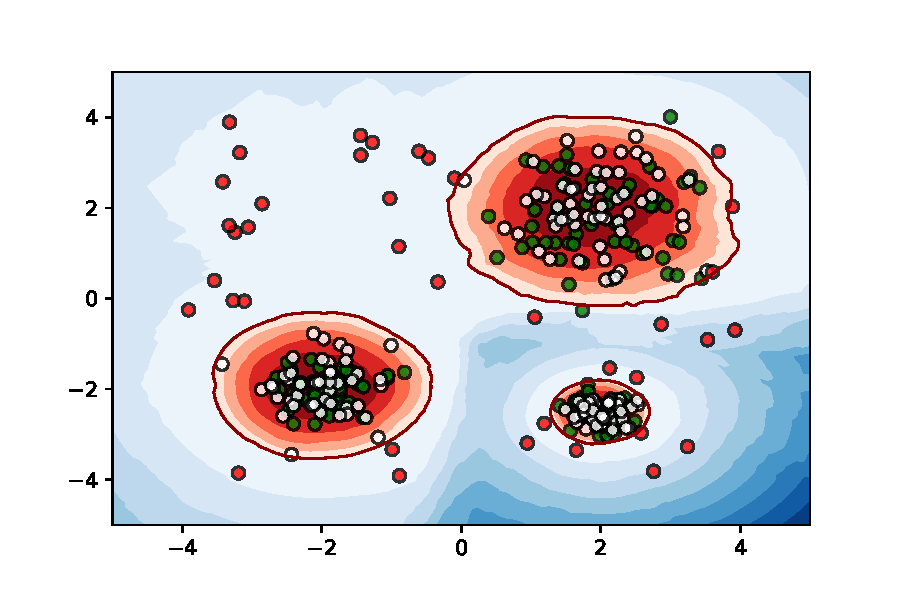
\includegraphics[width=0.48\textwidth,trim={12mm 5mm 15mm 10mm},keepaspectratio,clip]{figures/200-background-lof.pdf}
	\caption[Visualisation of the Local Outlier Factor]{Visualisation of the \gls{lof} in a 2 dimensional vector space. \emph{Green}: trainings data, \emph{Red}: outlier from test data, \emph{White}: inlier from test data. Background indicates the calculated \emph{LOF} value.}
	\label{fig:background:network:novelty:lof}
\end{wrapfigure}

Another proximity based approach to outlier detection is the \glsfirst{lof}, introduced by \textcite{Breunig2000}. It is based on the \gls{knn} problem, but accounts for locality and is specifically designed for outlier detection.
With \gls{lof} an outlier is a data point which \emph{MinPts} nearest neighbours are further away then these neighbours from each other. 
Using this lemma, For each data point the degree of \enquote{outlier-ness}, or local outlier factor, is determined.

By not relying on a global threshold, the \gls{lof} can account for clusters of different density. Therefore, one could argue, that the \gls{lof} is not only proximity based, but rather density based. Further by not treating the classification of an outlying observation as a binary property, analysis made on top of the outlier classification can be more precise. \parencite[cf.][]{Breunig2000}

Moreover, the ability of \gls{lof} to work on unclean data and account for different density in clusters through locality, making it a good match for \gls{ids} solutions, as \textcite{Lazarevic2003} shows. Also \textcite{Zanero2004} conducted an experiment on using unsupervised learning algorithms for intrusion detection and found, that the problem of locality with \gls{knn} has to be addressed in order to be more precise in predictions, what \gls{lof} archives.

\todo{ref to fig}

\subsubsection{Support Vector Machines}
\label{sec:background:network:novelty:svm}

\begin{comment}
	\begin{itemize}
		\item \enquote{The task of classification is to find a rule, which, based on external observations, assigns an object to one of several classes} \parencite{Muller2001}
		\item separate vector space by decision surfaces, setting boundaries between categories \parencite{Muller2001}
		\item \enquote{a learning algorithm for problems which are separable by hyperplanes} \parencite{Scholkopf2001a}
		\item \enquote{among all hyperplanes separating the data, there exists a unique optimal hyperplane, distinguished by the maximum margin of separation between any training point and the hyperplane} \parencite{Scholkopf2001a}
		
		\item One Class SVM
			\begin{itemize}
				\item aka. novelty detection
				\item all training data is considered good
				\item decision surface is fitted as close as possible to the training data
				\item new data outside this area, surrounded by decision surfaces, is considered an outlier
				\item \enquote{[...] does not require training data to be labelled to determine a decision surface.} \parencite{Lazarevic2003} (seems to be not exactly One-Class SVM)
				\item 
			\end{itemize}
	\end{itemize}
\end{comment}

\begin{wrapfigure}{l}{0.5\textwidth}
	\centering
	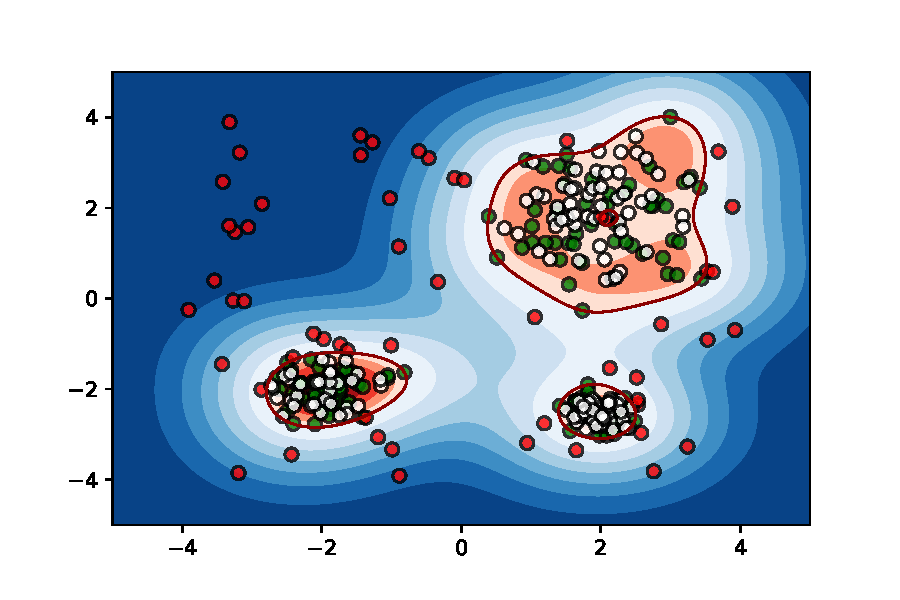
\includegraphics[width=0.48\textwidth,trim={12mm 5mm 15mm 10mm},keepaspectratio,clip]{figures/200-background-oneclass.pdf}
	\caption[Visualisation of a Support Vector Machine]{Visualisation of a \gls{svm} in a 2 dimensional vector space. \emph{Green}: trainings data, \emph{Red}: outlier from test data, \emph{White}: inlier from test data. Background indicates the distance from the decision surface.}
	\label{fig:background:network:novelty:svm}
\end{wrapfigure}

Another technique to discriminate outliers from \emph{normality} is to precisely model \emph{normality}, as \textcite{Hodge2004} described as third class of outlier detection algorithms. (cf. Section~\ref{sec:background:network:novelty:class})
\glspl{svm} are a widely used technique in this field. Especially one-class \glspl{svm} are applied in outlier and intrusion detection. \parencite[cf.][]{Lazarevic2003,Eskin2002}
They classify data points by defining decision surfaces within the feature space, which separate categories. A learning algorithm fits these hyperplanes to prior labelled data, basically finding a rule to separate data points into different classes. 
In case of one-class \gls{svm}, which are predominantly used for outlier detection, there is only one category resembling \emph{normality}. Hence the training data must contain the full gamut of normal data points, without any contamination introduced by anomalies. \parencite[cf.][]{Muller2001,Scholkopf2001a}

As \textcite{Eskin2002,Lazarevic2003} showed, \gls{svm} are a good and viable techniques to be used in anomaly-based \glspl{ids}. However, since the way this model is trained requires for clean training data, it is increasingly hard to fit it into new networks and changing environments. (cf. Section~\ref{sec:background:network:ids:anomaly})

\todo{ref to fig}

\begin{comment}
\subsubsection{Isolation Forest}
\label{sec:background:network:novelty:isoforest}
	
	\begin{itemize}
		\item \enquote{explicitly isolates anomalies rather than profiles normal instances} \parencite{Liu2008}
		\item \enquote{takes advantage of two anomalies’ quantitative properties} \parencite{Liu2008}
			\subitem \enquote{they are the minority}
			\subitem \enquote{have attribute-values that are very different}
	\end{itemize}
\end{comment}

\subsubsection{Entropy-based Outlier Detection}
\label{sec:background:network:novelty:entropy}

The information entropy, introduced by \textcite{Shannon1948}, provides an effective way to determine the uncertainty of a given system or the information content of a variable. It is further also referred to as measurement for randomness. Especially later one is intuitively related to outlier detection.

\textcite{Toshniwal2014} are using these characteristics and propose an algorithm to cluster data streams and determine outliers. 
The basic principle is to try to fit every occurring data point to every existing cluster. The data point is then finally assigned to the cluster, where it produces the least increase of entropy. Finally, the relative change of entropy for assigning a data point to the nearest cluster (\emph{PCE}) is calculated. If this \emph{PCE} is higher than a prior defined threshold, the data point is considered an outlier.
However, this method requires access to all previous data points, which implies a high resource utilisation. To increase performance \textcite{Toshniwal2014} are only keeping a window of data in memory.
Further, it might be to consider to determine a kernel function, fitted to the individual dimensions. The entropy could then be calculated against the distribution function, rather than raw data.

\begin{comment}
\subsection{Elliptical Envelope}
\label{sec:background:network:novelty:envelope}
	
	\begin{itemize}
		\item tries to fit data to estimated \emph{shape}
		\item does not seem to be a good match, since it required to know the distribution of the vector fields
	\end{itemize}

\subsection{Statistical techniques}
\label{sec:background:network:novelty:stat}

\begin{itemize}
	\item "Some [...] are applicable only for single dimensional data sets" \parencite{Hodge2004}
	\item "requires no user parameters as all parameters are derived directly from data" \parencite{Hodge2004}
	\item e.g. "Grubbs’ method (extreme studentized deviate) (Grubbs, 1969) which calculates a Z value as the difference between the mean value for the attribute and the query value divided by the standard deviation for the attribute where the mean and standard deviation are calculated from all attribute values including the query value. The Z value for the query is compared with a 1\% or 5\% significance level" \parencite{Hodge2004} also cf. \textcite{Grubbs1969}
\end{itemize}

\subsection{Proximity-based techniques}
\label{sec:background:network:novelty:prox}

\begin{itemize}
	\item "no prior assumptions about the data distribution" \parencite{Hodge2004}
	\item "not feasible for high dimensionality data sets" \parencite{Hodge2004}
\end{itemize}	


%\subsection{Bayesian}
%\subsection{Pattern Matching}
\subsection{Autoassociative Kernel Regression (AAKR)}
	used by \textcite{Yang2006}
\end{comment}

%\section{Time-based Anomaly Detection}

\subsection{Methods of Feature Encoding}
\label{sec:background:network:features}

Most algorithms and techniques for Outlier Detection (cf. Section~\ref{sec:background:network:novelty}) work within a multi-dimensional vector space or feature space. Often it is not straight forward to map specific features of a data set into a vector space.
Problematic cases included when the possible expressions of a feature need to be model as equidistant to each other.
Alternatively, in certain cases it is necessary to reduce the amount of dimension a feature would add, because otherwise the resource utilisation would exceed sane boundaries.

\subsubsection{One-Hot Encoding}
\label{sec:background:network:features:onehot}

Certain features in a dataset can represent markers or flags. In traditional data processing flags are often encoded as bit-field, where each bit represents one specific flag or marker, or as numerical value, where each number represents a state.
When using machine learning techniques, like Outlier Detection, directly on bit-fields or numerical encoded flags, a problem arises, especially with proximity base approaches.

For instance the \gls{apci} value encodes the application type in a \gls{knx} telegram as numerical value. (cf. Section~\ref{sec:background:bas:knx:communication})
For instance a \code{A\_GROUP\_VALUE\_WRITE} telegram is encoded with a value of \code{128}, whereby an \code{A\_GROUP\_VALUE\_READ} is encoded with a value of \code{000}, and \code{A\_INDIVIDUAL\_ADDRESS\_WRITE} with \code{192}.
The euclidean distance between those different \gls{apci} values would be 128, 64, and 0, which would indicate some kind of hierarchy or order.

However, for the sake of determining outliers, it is only of relevance if these values differ, the possibly induced hierarchy or order does not provide any information.
In other words the different expressions of this feature must be kept equidistant to each other.

To archive this, it is suggested in literature, to encode each expression as own dimension and only setting the expressed one to 1, leaving the rest at 0. This is referred to as \emph{one-hot} encoding. \parencite[cf.][]{Coates2011}

\subsubsection{Feature Hashing}
\label{sec:background:network:features:hashing}

When introducing multiple features in the vector space, the  amount of dimensions can increase rapidly, especially when using techniques like one-hot encoding (cf. Section~\ref{sec:background:network:features:onehot}).
This has huge implications with regards to resource consumption and more importantly to the feasibility of used algorithms on the vector space.
For instance proximity based approaches to Outlier Detection do not perform well in high dimensional vector spaces. \alert{cite needed}

To reduce the number of dimensions the amount of features could be reduced, or one could compress the feature vector. One method to archive compression by maintaining the informative value is called Feature Hashing or Kernel Trick. \parencite{Weinberger2009,Shi2009}
As the name suggests a specialised hash function is applied to the feature value to reduce the required dimensions down to a defined size.
This process is non reversible, which might have implications for further processing the results, e.g. using the coordinates of decision planes in \glspl{svm}.
Further, feature hashing introduces the possibility of hash collisions, especially when the targeted dimension number is low. Therefore the reduction needs to be considered carefully.
However, when compared to a random projection, to reduce dimensionality, the hashing-trick preserves the density and introduces no additional overhead. \parencite{Weinberger2009,Shi2009}

\subsubsection{Encoding Time}
\label{sec:background:network:features:time}

Encoding time in machine learning and in the context of anomaly detection has to be considered carefully.
First, time can not be simply expressed as \gls{unixts}, since it is not recurring by design, therefore providing no point to correlate future data points to.
As a consequence. time has to be within a seasonal context. This can be a week, a year, or any other season time range, in which events reoccur.
For example, human behaviour tends to organised in a weekly rhythm. This would make a week our reoccurring cycle. Within this cycle one could express time as seconds since the beginning of the week, e.g. Monday 00:00, and normalised against the length of a week in seconds.

Another approach on how to incorporate time could be to train several models, each one representing a fraction of the seasonal cycle. For instance, the week could be divided by days, and there would a model for Monday, a model for Tuesday, etc. pp.
However, doing this might introduce problems at the transition points between those models. So might an action which in the training set never occurred on a Monday, but always on Tuesdays only a few minutes past midnight, be considered an outlier simply due to the fact that it never happen to be trained in the Monday model.
The overall consequence is, that a few minutes in timing can change the decision surface dramatically, which is used to determine the \emph{normality.}

To mitigate these drawbacks, one could train the double amount of models, but with half of them shifted by half a time step. This would result in 14 models in our example. The first half would be normal day models, reaching from midnight to midnight. The second half, however, would be shifted by 12 hours and therefore reaching from noon to noon.

\todo{include fig from concept}

\begin{comment}
\begin{itemize}
	\item use feature direct as vector-dimension (not so good)
	\item OneHot encoding
		\subitem one vector-dimension per possible feature vector
		\subitem if feature has specific value, set dimension for this value to 1, the rest 0
		\subitem also cf. \textcite[][p. 12]{Eskin2002}, not mentioned as term, but good math-like description
		\subitem reversible
	\item Feature Hashing / Hashing Trick
		\subitem defined amount of dimensions
		\subitem feature value is hashed
		\subitem hash value is then used
		\subitem non reversible
		\subitem possibility of hash collision
		\subitem esp. when dimension count is low
		\subitem \enquote{\emph{hashing-trick:} one hashes high dimensional input vectors $x$ into a \emph{lower} dimensional feature space $\mathbb{R}^m$ with $\phi: X \rightarrow \mathbb{R}^m$} \parencite{Weinberger2009,Shi2009,Langford2007}
		\subitem \enquote{Different from random projections, the hashing-trick preserves sparsity and introduces no additional overhead to store projection matrices} \parencite{Weinberger2009}
	\item "normalize all [...] attributes to the number of standard deviations away from the mean." \parencite{Eskin2002}
		\subitem "scale based on the likelihood of the attribute values" \parencite{Eskin2002}
\end{itemize}
\end{comment}
	
	%\chapter{Prior Work}
	\clearpage
	\section{Prior Work in Anomaly Detection for BAS}
	% what does exits already
	\label{sec:background:prior-work}
	% !TeX spellcheck = en_GB

%\section{Prior Work and Existing Solutions}
%\label{sec:background:network:priorwork}

\begin{itemize}
	\item \parencite{Yang2006}
	\item \parencite{Celeda2012}
	\item \textcite{Pan2014} BACnet
	\begin{itemize}
		\item Anonmaly detection for BACnet fire alarm systems
		\item taps BACnet traffic via IP
		\item rule based learning (RIPPER)
		\item protection against common BACnet attack vectors
		\subitem who-is/who-has network probing
		\subitem write-property (take control over device)
		\subitem InitializedRoutingTable
		\subitem reinitialize devices
		\subitem application layer DoS
		\subitem flooding of network
	\end{itemize}
	
	\item \textcite{Eskin2002} algos for unsupervised anomaly detection in IDS
	\item \textcite{Leung2005} Unsupervised anomaly detection in IDS, proposed new algo \emph{pfMAFIA}
\end{itemize}

Despite being widely used and applied in \gls{ip} networks \parencite[cf.][pp.~201~ff.]{Northcutt2005}, \gls{ids} seem rather seldom utilized to monitor \glspl{bas}.
However, there are a few examples in literature where the principles of \glspl{ids} are applied to \gls{scada} and \gls{ics}.


	
	\chapter{Methodology}
	% what methods do I use (experiments, hard thinking, not so hard thinking, etc.)
	\label{sec:methods}
	% !TeX spellcheck = en_GB

\begin{comment}
\begin{itemize}
	\item experiment
	\item test data captured from a floor section of the computer science building
	\item enriched with malicious packets to keep consistent
	
	\item (focusses only an purpose based) attack classes (cf. \parencite{Uma2013})
		\subitem \gls{dos}
			\subsubitem Short circuit -> blackout on entire line
			\subsubitem flooding of \code{A\_Restart} telegrams
			\subsubitem flooding nonsense
		\subitem replay
			\subsubitem repeating a time window
			\subsubitem sniff a tag and repeat it compressed??? \alert{whatever this means?}
			\subsubitem do inverse action
		\subitem manipulation/reconfiguration
			\subsubitem telegram manipulation
			\subsubitem reconfiguration of devices (Access Attack)
			\subsubitem reconfigure line couplers/make them useless (Access Attack)
		\subitem spoofing 
		\subitem Reconnaissance Attack
			\subsubitem network mapping
			
		\subitem 
	
	\item aim is to show if attacks can be identified by anomaly detection on flow data
		\subitem under the assumption, that attacks noticeable alter the characteristic and behaviour of \gls{knx} traffic
		\subitem cf. \parencite{Mukherjee1994,Yang2006,Pan2014}
	\item demonstrate a message-passing architecture to perform online analytics on \gls{knx} flow-data
	\item benchmark different algorithms against each other
\end{itemize}
\end{comment}

The objective of this thesis is to investigate, whether anomaly based \glsfirst{ids} can provide additional security benefits for \glsfirst{bas} in the same they does for \gls{scada} networks. (cf. Section~\ref{sec:intro})
Given the assumption, that every malicious activity or attack within a network induces noticeable different characteristics and behaviour, these deviations should be also identifiable in aggregated flow-data of this network. \parencite[cf.][]{Mukherjee1994,Yang2006,Pan2014}
For this I designed a message-passing architecture to test different established algorithms for anomaly detection using flow-data from \gls{bas} networks.

The test will be conducted as an experiment with data captured in a floor segment of the computer science building over the course of one month. \alert{check, if I can get a second month for verifying the training?} It is assumed, that this data set does not contain any malicious activities.
Consequently, this data will be used to train multiple models using different algorithms.
Then a comparable data set is used to ensure that the models are not over-fitted and do not raise alarms during normal operations.
Further, the same validation data set is modified with malicious activities, which might be cause by a range of plausible attacks scenarios.
This, in turn, is down to ensure that the models and algorithms are not under-fitted and are suitable to detect anomalies, which might be induced by malicious activities.
However, the experiment will not focus on determining, if the system can distinguish between malicious abnormal activities and legit abnormal activities, which might be caused by a rapid change of user behaviour. In this thesis both are considered worth reporting.

Mostly since rapidly changed user behaviour is difficult to simulate in our test case, the actual test and benchmarking will be done using a set of plausible attacks. \hint{Is this even the right place to describe the attacks?}
These attacks include \emph{\glsfirst{dos} attacks}, which can be induced by multiple action: First of all shorting the line circuit would effectively causing a communication blackout on the entire line. Also flooding \code{A\_Restart} telegrams to all devices, would render the devices useless, since they would be stuck in a restart loop. As last scenario of \gls{dos} attacks, flooding the line with non-sense telegrams on high priority (cf. Section~\ref{sec:background:bas:knx:proto}) would cause at least heavily delayed, if not entirely blocked, normal communication on the line, since no time window would be left open for normal priority telegrams.

Another plausible attack scenario would be replay attacks, where 3 flavours might be imaginable.
In the first case an attacker would captures traffic for a determined time span and then replays it on the network, possibly to mimic normal behaviour while breaking into the building.
Secondly, an attacker could capture an specific event and replay it on will, which could the command to open an security door for instance.
As a third option, the traffic could be monitored and for every action an reverse action could be invoked, effectively keeping the \gls{bas} in one state. The simplest example would be, to turn off the lights every time somebody tries to turn them on.

The next category of attacks can be classified as manipulation or reconfigure attacks. This includes attacks which might modify telegrams while they are send, to either render them invalid and therefore preventing communication. Or it would be conceivable to reconfigure devices, i.e. to trigger different actions, report false measurements etc. A specialisation of this attack focusses on line couplers and breaking the network segmentation by disabling any routing functions.

Finally, the last category describes reconnaissance attacks, which focus on unauthorised detection and mapping of the network. Here only active sweeping approaches are considered, since passive eavesdropping can not be detected on higher protocol level due to the bus character of the network. (cf. Section~\ref{sec:background:bas:knx:topo})

\hint{check plausibility of this}
\todo{write more about evaluating the results?}
For each category of attacks, the different anomaly detection algorithms are benchmarked with regards to their detection rate.

\begin{comment}
Angriffe:

DoS
	Kurzschluss im Bus -> DoS auf gesamtem Segment
	A_Restart-Pakete -> DoS gegen einzelne Teilnehmer
Replay-Angriffe
	Zeit mitschneiden -> wiedergeben
	Tag mitschneiden, komprimiert wiedergeben
Manipulation von Paketen (Payload tauschen)
Konfiguration manipulieren
Überwindung von Linienkopplern
Address-Spoofing
	falsche Adresse in Liniensegment
	mit existierender Adresse senden
Netzanalyse mit knxMap (https://github.com/takeshixx/knxmap)
Mitlesen und sofort gegenteilige Aktion auslösen
High-Level-Angriffe:
	nur best. Aktionen zulassen
	Provokation/Sabotage von menschl. Verhalten
Social-Engineering -> Einschleusen von Geräten
\end{comment}
	
	%\chapter{Conceptual Architecture}
	\chapter{Concept of an Intrusion Detection System for BAS}
	\chaptermark{Concept}
	% concept
	\label{sec:concept}
	% !TeX spellcheck = en_GB

\begin{comment}
\begin{itemize}
	\item goal == identify threats/attacks in KNX networks
	\item only a part in defence system
	\item attempt is to fit anomaly detection model best to normal behaviour in the network
	\item therefore it also necessary to account for usage cycles/periods/seasons of building usage
	\subitem since it has a direct impact on the bus activity
	\item changes in usage may be identified as anomaly -> which could also be interesting
	\subitem reflect e.g. physical intrusion, not intended use of the building, etc.
	\item ...
	
	\item novelty == in-band monitoring
		\subitem mention problems
	\item basic architecture according to \textcite{Pan2014}
	\item \enquote{Intrusion detection systems (IDSs) “are based on the beliefs that an intruder’s behavior will be noticeably different from that of a legitimate user and that many unauthorized actions are detectable” [2].} \parencite{Mukherjee1994,Yang2006}
	\item focus on inside attacks \enquote{The intruder has been granted access to the network and may have some knowledge about the network architecture, including where their targeted files or system vulnerabilities.} \parencite{Yang2006}
	
	\item only high level anomaly detection is done by algorithms, since simple measurements can be evaluated in Grafana
		\subitem e.g. change in packets per seconds
\end{itemize}
\end{comment}

\todo{better intro sentence?}
The overall goal is to identify and react to threats and attacks within \gls{bas} networks, which are indicated by malicious traffic.
This thesis attempts to solve on part of the problem by providing a framework to detect anomalies in those networks.
However, it is not part of this concept to identify the kind of attack, nor to distinguish it from abnormal network activity, caused by a rapid change of user behaviour.
Also it is to note, that the introduced system is merely a part in the defence line.

The architecture proposed in this section is inspired by \textcite{Pan2014}, with extensions made in regards for scalability and continuous use. (cf. Section~\ref{sec:concept:pipeline})
Opposed to \textcite{Pan2014}, which are using an inductive rule learning algorithm (cf. Chapter~\ref{sec:background:prior-work}), this work employs anomaly detection algorithm, which are able to be trained with unlabelled data sets. (cf. Section~\ref{sec:background:network:novelty})
This decision was made because \gls{bas} are mostly heterogeneous, since every building and its usage is different, compared to the fire detection system used by \textcite{Pan2014}.
Therefore, either the baseline model has to reflect a very broad \emph{normality}, or attacks are modelled as signatures. Later option has the drawback of requiring constant updates. Also a sufficiently large database of common attacks is required in first place.
Neither of these options seemed feasible.
Consequently, relying on anomaly detection algorithms made more sense in the provided context.
Despite anomaly based \glspl{ids} being highly useful in changing environments with possibly unknown threats (cf. Section~\ref{sec:background:network:ids:anomaly}), it is to note that they \enquote{are based on the beliefs that an intruder's behavior will be noticeably different from that of a legitimate user and that many unauthorized actions are detectable}. \parencite{Mukherjee1994,Yang2006}

\todo{better transition}
Further, to enable scalability and on-line detection, the proposed framework was designed around the message-passing design principle.
This allows for an easily scalable deployment, strongly capsules application modules, and handles recovery after crashes without data-loss.
Especially later two are not only desired characteristics of an production system, but also speed up development and testing rapidly.

Another novelty, compared to prior examples in literature (cf. Chapter~\ref{sec:background:prior-work}), is the focus of passing the flow-data from the Agent to the collector in-band. By doing so, there is no requirement for additional network wiring, which results in easier and possibly cheaper deployment for Agents across the network.
However, this also introduces new challenges, as the aggregated flow data needs to fit within a relatively small data package, in case of \gls{knx} 255 Bytes. (cf. Section~\ref{sec:background:bas:knx:proto:data})
Also, the collector and the analytical modules need to account for the fact, that no traffic from the Agents can pass the network, e.g. due to \gls{dos} attacks.

\todo{challenge, since there are no real flows.}
Another challenge arises from the nature of \gls{bas} itself. Unlike \gls{scada} networks, where actions follow strict rules and orders and are therefore highly predictable or \gls{ip} networks, which mostly transport connection based traffic. The communication in \gls{bas} networks consists of many short self-contained commands, which occur in seemingly random fashion, since they are mainly triggered by human behaviour. This includes (light) switches, \gls{pir} motion detectors, or door sensors.
Due to the fact, that most telegrams are short commands or status reports from sensors, there are no elaborative connection based communication flows in \gls{bas} networks, thus rendering flow-monitoring less useful.
To counteract this \hint{somewhat special} characteristic, the idea of flow-monitoring is interpreter rather liberal. 
Namely, by focussing more statistics of all telegrams or packets during a specific synchronised time window, instead of tracking individual flows, which also requires less resources on the Agent.

As already mentioned, this system can merely be a part of comprehensive security system. Acknowledging this fact, the outlier detection algorithms focus mainly on high level anomaly detection, as simpler measurements, like a change in telegrams per seconds, can be simply evaluated in a monitoring and alerting frontend like \gls{grafana}.

\section{Monitoring Pipeline}
\label{sec:concept:pipeline}

\begin{itemize}
	\item goal == monitor KNX traffic
	\item notion of \emph{project} is used to differentiate unique, not comparable KNX networks. Can be seen as a common prefix for everything which need to be named internally.
	\item monitoring should include the whole network/world view
	\item monitoring needs to be distributed, so Line Couplers can be configured properly
	\item monitoring is done by Agents
	\item Agents will send data gather over a time window to the collector (ref to neflow terminology)
	\item time windows of Agents are synchronised (by the collector) to make data analysis more reliable
	\item Agents send gathered data to collector via KNX network
	\item collector stores windows immediately in InfluxDB
	\item collector checks regularly the InfluxDB, if all Agents send in their time window
	\item if so the collector relays all windows, describing the same time slot (+/- a couple seconds), to the analyser modules
	\item if not all windows are in by specified timeout (10s or so) they are relayed anyway
	\item bundled windows are distributed by pub-sub-server independently to different analytical modules
	\item analytical modules compare the windows to a base-line model (in different fashions)
\end{itemize}

For the overall goal to identify threats and attacks within \gls{bas} networks by detecting anomalies, a reliable way to monitor packets or telegrams within said networks is required. Further, this data needs to be processed and analysed, for which a data-pipeline seems well suited.
In this section the general structure and flow within this pipeline is presented. (cf. Figure~\ref{fig:concept:architecture})

Within the here proposed pipeline the notion of a \emph{project} is used to differentiate unique, not comparable \gls{bas} networks, which share the same analytical resources. It can be understood as common prefix for all internal references. (cf. Chapter~\ref{sec:impl})
This is not only a beneficial option, when monitoring multiple networks one the same analytical infrastructure, but also allows for quick testing with different data-sets during development.
%To further improve use in production, as well as ease of development, ... (RabbitMQ, but this a detail for impl sec)

Following concepts in literature \parencite[cf.][]{Celeda2012,Pan2014} the pipeline is not build around analysing a full-take of traffic within a \gls{bas}, but rather follows the flow monitoring idea. (cf. Section~\ref{sec:background:network:netflow})
However, as stated above (cf. Chapter~\ref{sec:methods},~\ref{sec:concept}), traditional flow monitoring is well suited for \glspl{bas} like \gls{knx}. Therefore, the focus is on general statistical data of all packets or telegrams passing by an Agent within a specific time window.

Since one of the requirements for sufficiently efficient flow-monitoring is to obtain world view (cf. Section~\ref{sec:background:network:netflow},~\ref{sec:methods}), multiple flow monitoring Agents need to be distributed across the \gls{bas} network. Otherwise, network segmentation would be required to be switched off, so a central tapping point could be used for data acquisition.
Whereas this would decrease complexity, it is not advisable since segmentation is one of the fundamental security concepts e.g. in \gls{knx}. (cf. Section~\ref{sec:background:bas:knx:security})
Consequently, a number of Agents, distributed over the whole network, will gather statistical data and send it of to central service -- the Collector.

The Collector is not only responsible for receiving data from Agents and storing them in a database, but also synchronises these windows. Synchronising the windows simplifies the implementation of the analytical modules (cf. Section~\ref{sec:concept:anal}), since they do not need to account for distorted weights, introduced by changing overlaps or lengths of windows sent by the Agents.
This is archived, first of all by waiting until all windows from all Agents have been send to the Collector. Only then they are relayed to the analytical modules as one unit.
However, this only works reliable if the Agents are in sync with each other. If not the Collector would need to compensate for different, changing overlaps. Therefore another task of the Collector service is to ensure the Agents are synchronised, meaning the Agents capture the same length of the of statistical data in the same rhythm without shifting. \alert{rhythm is quite the right thing here, it's more a shift of the length...}
This is archived by communicating back to the Agent modules, regularly updating the \gls{rtc} and important settings like window length and a time point for starting new windows. (shift in time)

Regular two-way communication between Agents and Collector also has the benefit of identifying simple replay attacks (cf. Section~\ref{sec:methods}), since not or wrongly reacting to configuration requests can be detected.
Further, accounting for dynamic configuration of the agents allows for adjusting parameters based on the general network load.
E.g. the Collector could prolong the window length, when the \gls{bas} network is under heavy load to reduce additional traffic. Or the Collector could do the exact opposite to receive more detailed information on heavy resource utilisation.




\todo{figure, that shows how Agents are distributed in the network?}
\begin{figure}[h]
	\centering
	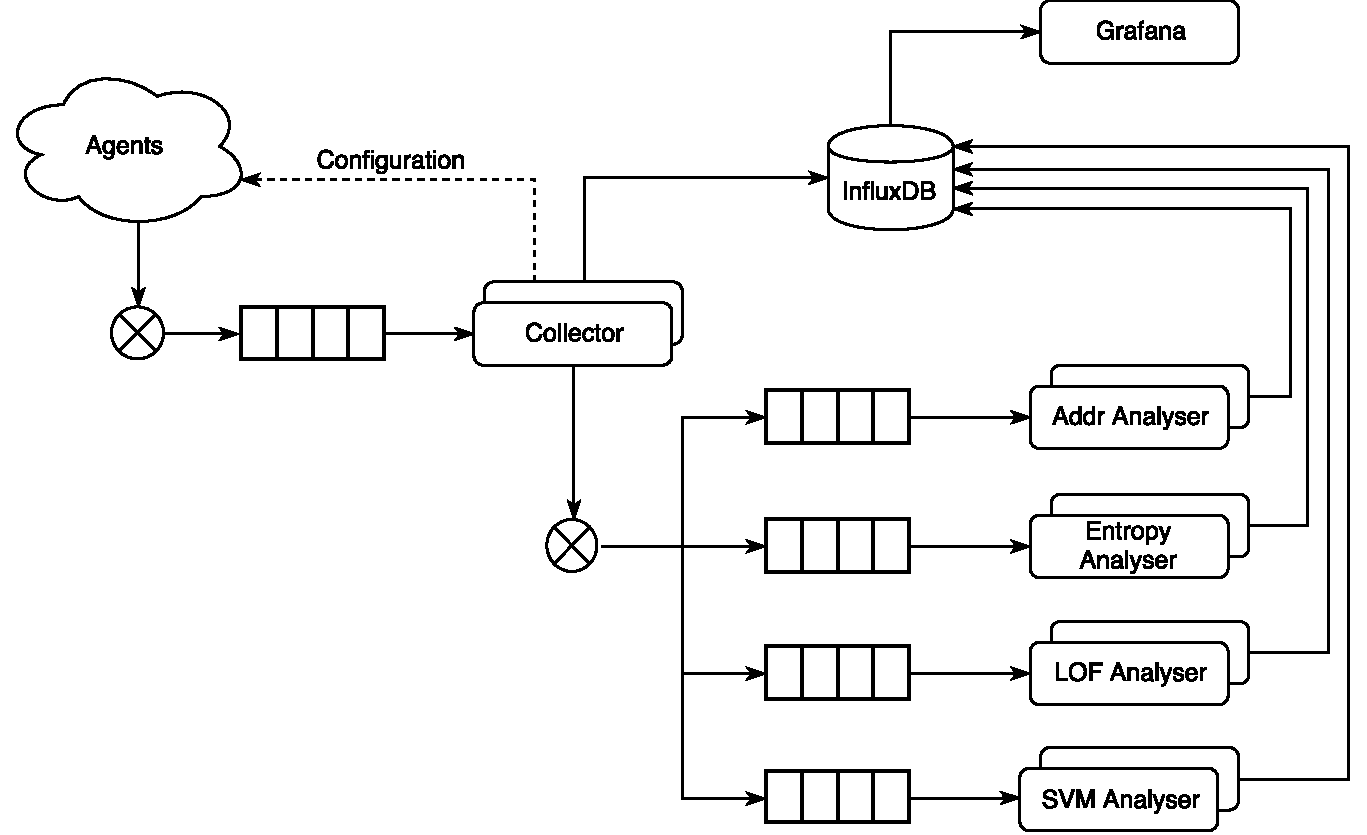
\includegraphics[width=\textwidth]{figures/300-concept-architecture.pdf}
	\caption[Pipeline Architecture]{Architecture of the monitoring pipeline \todo{explain symbols.} \todo{information flow back to agents, for time sync.}}
	\label{fig:concept:architecture}
\end{figure}

\section{Design of Netflow Agent}
\label{sec:concept:agent}

\begin{itemize}
	\item dedicated device
	\item sits in each or strategic important lines
	\item listens to bypassing traffic and aggregates it
	\item \alert{Critical to describe the difference to original netflow concept/idea here and why this decision was made}
		\subitem netflow is very IP oriented, where protocols include normally connections (TCP) or at least multiple steps/packets
		\subitem this provides a basis on which aggregation/grouping can be performed
		\subitem basically no flow (multi step protocols) in \gls{knx} during normal operation (besides configuration phase in \gls{knx})
		\subitem therefore gather statistical distribution of features on \gls{knx} \gls{telegram} over a given time span (window length)
		\subitem time span/window length should be configurable by the collector, so it can be adjusted according to network utilisation
		\subitem window length still needs to be synchronised among all agents to be able to use all aggregated agent windows in a world model
		\subitem further \gls{knx} can only transport 255 Bytes max in one telegram -> serious size restrictions
	\item after timeout gathered/aggregated data is send via \gls{knx} \gls{telegram} to the collector
	\item window consists
		\subitem meta data (timestamps, window lengths)
		\subitem absolute counter of how often an specific feature appeared in a window
			\begin{itemize}
				\item specific source address
				\item specific destination address
				\item apci value
				\item a specific payload length
				\item a specific \gls{hops}
			\end{itemize}
		\subitem checksum, and possibly signature
	\item window is encoded in a binary format to fit in the 255 Bytes
\end{itemize}

\section{The Collector Module}
\label{sec:concept:collector}

\begin{itemize}
	\item responsible for
		\subitem collecting data from agents through the \gls{knx} network
		\subitem storing raw time windows in \gls{influxdb}
		\subitem relaying raw, synchronised time windows to analytical modules
	\item listens to a single message queue containing time windows from all agents assigned to the same project
	\item agents must have unique names within one project
	\item windows are parsed and then submitted into the \gls{influxdb}, tagged with the agent-name and the project
	\item window is split into different measurements (tables) determined by the \gls{knx} fields observed.
	\item one additional measurement (table) \code{agent-status}, representing general status information
		\subitem timely length of the window
		\subitem end timestamp of the window
		\subitem boolean if window was relayed or not
	\item collector regularly checks the \gls{influxdb} for unrelayed windows (latest ones first)
	\item windows are grouped by time slot
	\item if all agents have submitted a window for a specific timeslot these windows are bundled and relayed to the analyser message exchange (cf.~Figure~\ref{fig:concept:architecture})
	\item for all successfully relayed windows set the \code{realayed} flag in the \code{agent-status} measurement to \code{true}
\end{itemize}

\section{Analyser Modules}
\label{sec:concept:anal}

\begin{itemize}
	\item 2 phases
	\item distinguished learning phase
	\item during learning phase the analyser module accesses directly the \gls{influxdb} for a specified time range
	\item group windows by time equal to the functionality of the collector
	\item construct \gls{vect} to train base model
	\item save base model in the filesystem
	
	\item during normal (analytical) operation
	\item accept grouped windows from collector via message exchange
	\item compares current window groups to base model to detect anomalies
	\item results of this analysis are stored back into the \gls{influxdb} as a separate \gls{idbmeasurement}
	
	\item multiple anomaly detection algorithms were considered
	\item according to \textcite{Lazarevic2003} \gls{lof}, NN, and unsupervised SVM perform the best
	\item \textcite{Eskin2002} suggests clustering and SVM as best performing algorithms
	\item ...
\end{itemize}

\subsection{The Address Analyser}
\label{sec:concept:anal:addr}

\begin{itemize}
	\item purpose is to detect new (novel) device addresses
	\item cf. new device attack
	\item during the learning phase it logs all occurring source and destination addresses per agent
	\item in the analytical phase it compares all source and destination addresses in a window with addresses (base model) accumulated in the training phase
	\item output \glspl{idbmeasurement}: \code{unknown\_src\_addr}, \code{unknown\_src\_telegrams}, \code{unknown\_dest\_addr}, \code{unknown\_dest\_telegrams}, \code{unknown\_addr}, \code{unknown\_telegrams}
\end{itemize}

\subsection{The Local Outlier Factor Analyser}
\label{sec:concept:anal:lof}

\begin{itemize}
	\item cf.~Section~\ref{sec:background:network:novelty:lof}
	\item proximity based technique (cf.~Section~\ref{sec:background:network:novelty:prox})
	\item tries to determine if a window represents normal behaviour
	\item both for local and world view
	\item builds feature vector out of
		\subitem normalized seconds since the beginning of the year
		\subitem source addresses
		\subitem destination addresses
		\subitem priority distribution
		\subitem hop count distribution
		\subitem payload length distribution
		\subitem \gls{apci} usage distribution
	\item time sensitivity/seasonal sensitivity is archived by including the relative timepoint in the current year
	\item training different model for different seasons is not necessary since \gls{lof} is a proximity base approach
\end{itemize}

\subsection{The Entropy Analyser}
\label{sec:concept:anal:entropy}

\begin{figure}[h]
	\centering
	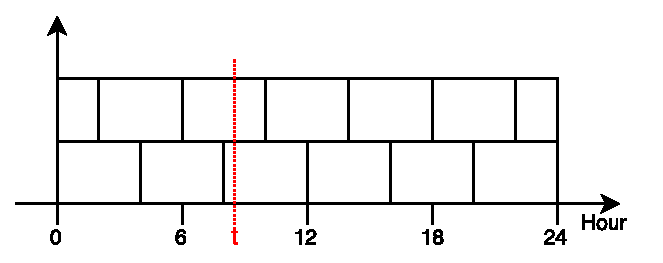
\includegraphics[]{figures/300-time-slots.pdf}
	\caption{Example of shifted time slots used in the entropy analyser module.}
	\label{fig:concept:time-slots}
\end{figure}

\begin{itemize}
	\item cf.~Section~\ref{sec:background:network:novelty:stat}
	\item statistical approach
	\item base model is trained using distribution of the \gls{pmf}
		\subitem determine statistical distribution per dimension in feature vector
	\item determine distribution for local (per agent) and world view
	\item to incorporate different seasons multiple base models are trained 
	\item the seasonal time range (day, week, year) is separated into slots
	\item amount of slots is doubled with half a slot length offset, so 2 slots apply per time point cf. Figure~\ref{fig:concept:time-slots}
	\item mitigates issues with artificial break on slot change
	\item feature vector
		\subitem source addresses
		\subitem destination addresses
		\subitem priority distribution
		\subitem hop count distribution
		\subitem payload length distribution
		\subitem \gls{apci} usage distribution
	\item entropy/information gain is calculated for the current distribution of the feature vector compared to the respectively base model
	\item individual entropies are summed up and stored in the \gls{influxdb} (additional to the individual entropies)
\end{itemize}

\section{Monitoring and Alerting}
\label{sec:concept:mon}

\begin{itemize}
	\item using \gls{grafana}
	\item visualise basic time series like amount of packets per agent
	\item visualise and monitor output from analyser modules
		\subitem should stay below certain threshold
	\item use internal alerting function
	\item benefits
		\subitem use existing, proven solution
		\subitem gain features for free (auth, alerting, graphing, etc)
		\subitem integrate with metrics from other sources
	\item decoupled from analyse modules
	\item good integration with \gls{influxdb}
\end{itemize}

	
	\chapter[Implementation of a Prototype]{Implementation of a Prototype IDS for BAS}
	%\chaptermark{Prototype Implementation}
	\label{sec:impl}
	% !TeX spellcheck = en_GB

\begin{comment}
\begin{itemize}
	\item implementation in \gls{py} 3
	\item command line interface with subcommand as central entrypoint providing configuration and log management
	\item each process is run as separate processes to mitigate \gls{gil} limitations
	\item process has one task (agent simulator, collector, analyser module)
	\item modules/process pass messages mainly using \gls{amqp} and \gls{rabbitmq} as message broker
	\item reusing \gls{influxdb} and \gls{rabbitmq} by separating pipelines using a project name
\end{itemize}
\end{comment}

To validate, test, and proof the concept as described in Chapter~\ref{sec:concept}, it was implemented as prototype using \gls{py}3 and the \gls{sklearn} library for data analysis.
The working name for the prototype is \emph{BAS Observe}, or short \emph{BOb}.
As the concept evolves around a message-passing architecture, the prototype follow this approach as well by using \gls{amqp} with \gls{rabbitmq} as message-broker. As central data storage the time-series database \gls{influxdb} is used, since it provides good querying capabilities and excellent integration with existing third-party solutions like \gls{grafana}, which will be used as monitoring and alerting solution.

This enables to run the various modules as separate processes on possibly different machines, as every message exchange is done via the message-broker and historical data can be queried directly form the database.
As a side effect the possible restrictions introduced by \gls{py}s \glsfirst{gil} are circumvented.
Even though each module is capsuled in an own process, all of them can be started using an unified \gls{cli}, which abstracts things like configuration and logging, as well as connection management for the \gls{amqp} message-broker and the database.
For interacting with the \gls{rabbitmq} message-broker \gls{lib-pika} 0.11 is used. To query from and push values to the \gls{influxdb} time series database the official \gls{py} client side library is used.
The implementation details of each module are described in-depth in the following sections.

\section{The Command Line Interface}
\label{sec:impl:cli}

\begin{comment}
\begin{itemize}
	\item central entry point for all operations
	\item consistent user experience -> less fiddling while debugging/developing
	\item centralises configuration and log setup
	\item can be easily made accessible via python setuptools
		\subitem if globally installed, callable via normal terminal command
	\item implemented using the \gls{lib-click} library version 6
\end{itemize}
\end{comment}

The \glsfirst{cli} provides a central and consistent entry point for all operations and is implemented using \gls{lib-click}, which provides an fast way to define command line options and parameters with code annotations.
The \gls{cli} can be installed via \gls{py} setup tools and exports one command into the operating system's search path, called \code{bob}.
This exported main command does not provide any functionality itself, apart from taking basic configuration parameter like the database and message-broker host, log level, and a project identifier -- all of which are preset to sane defaults.
Rather the command exposes a series of subcommands.

The first being \code{bob collector}, which invokes the collector module and only requires a list of available agents additionally to the basic configuration and is further described in Section~\ref{sec:impl:collector}.
Besides the Collector an agent simulator can be invoked by \code{bob simulate}, which can simulate multiple Agents from the content of a \gls{knx} log file, as described in Section~\ref{sec:impl:agent}.
By only on replaying existing observations an controllable and repeatable test environment can be archived. An Agent implementation able to process live traffic was not considered necessary for the point of demonstrating and testing the proposed concept.

The Analyser modules, however, can be invoked by either two generic subcommands, \code{bob train} which starts a module in training mode or \code{bob analyse} which runs the module in the operational, analytical mode.
All training commands take tree additional parameters: a start and end time of the period to be used as training data and the path to a model file, where the training results can be stored. The module which is supposed to be trained can be selected by adding it as another subcommand, so would \code{bob train lof} start the training mode of the \gls{lof} Analyser.
Same applies for the operation mode, where, however, the start and end date can be omitted and only the path to a model file needs to be passed. So can the Address Analyser be called by \code{bob analyse addr}.

Additionally to starting modules, the \gls{cli} implementation also takes care of configuration management and logging.
Despite being not critical for demonstrating the performance of the implemented concept, a consistent, easy, and documented mechanism for running modules eases development and hopefully will increase the reuse-ability of the source code.
A feature that deliberately was left out were configuration files. For the purpose of showcasing the concept it did not seem necessary and comes with the risk of hiding configuration parameter out of sight, which possibly increases the risk of mistakes made just because a changed parameter was forgotten. By plainly relying on command line parameters for configuration, the configuration is always in plain sight, when invoking a command.

\todo{explain 'project' notion}

\section{The Collector Module}
\label{sec:impl:collector}

\begin{comment}
\begin{itemize}
	\item central hub for relaying information
	\item receives agent windows via \gls{amqp} message broker (cf. Figure~\ref{fig:concept:architecture})
	\item subscribed to the agent topic using \gls{lib-pika} version 0.11
	\item incoming windows from agents are stored immediately in \gls{influxdb}
	\item every 4 seconds a callback \hint{(other word for callback?)} is called
	\item callback queries \gls{influxdb} for not relayed windows
		\subitem ordered latest first
		\subitem so a cumulating backlog does not affect the ability to show/process near-real-time metrics
		\subitem old windows will be processed once backlog decreases
	\item collector groups windows by timeslot
		\subitem so analysers receive a snapshot of the network
		\subitem allows them to analyse world-view without the need to compensate time-difference
\end{itemize}
\end{comment}

The central hub for relaying and transforming information is implemented in the Collector module.
It receives \gls{json}-encoded windows with statistical data from Agents by subscribing to an \gls{amqp} topic on the message-broker. Each incoming window is parsed, checked for format errors, and then immediately converted into a format suitable for \gls{influxdb} and pushed to the database. Only then the processing of the window is acknowledged to the message-broker, which ensures that no windows is dropped in cases Collector implementation crashes. This is archived by relying on retry functionality of message queues in the \gls{rabbitmq} broker and only requesting one message at a time.

Additionally, the Collector relays all windows belonging to one time slot to the Analyser modules, once one window from each Agent is written to the database.
For this a callback is invoked every $4$ seconds, which queries the $50$ latest, not relayed windows from the database. Whereby only the management measurement is queried containing the window length, star and end time, and relayed status, to reduce the size of data that needs to be handled.
These windows are then sorted into a hash-map of time slots, where the key is the averaged timestamp of all windows in this slot. The idea is to allow a certain degree (up to $2$ seconds) of clock drift in the Agents. 
So, if a window is added to the hash-map, a loop iterates over all existing keys and returns the key closest to the timestamp of the window, but with a maximum delta of $2$ seconds.
The window is then added to that timeslot and the key is recalculated as the average of all window timestamps in this slot, including the newly added one.
If no timeslot within $2$ seconds around the window exists, a new one will be created with the window's timestamp as key.

Once all queried windows are sorted into the hash-map, the Collector checks if a time slot contains windows from all Agents, by validating against a configurable list of Agent-ids.
When the time slot is complete, the windows are enriched by querying all remaining measurements from the database and then relayed to the Analyser modules via an \gls{amqp} message exchange, which distributes it into multiple message queues.
Only if the windows were successfully passed into to the message-broker, they are marked as relayed in the database. This ensures, that every window is processed. However, this way can not prevent time slots to send repeatedly to the Analyser modules, if the Collector crashes right before marking them as relayed in the database. In contrast to receiving windows form Agents and initially writing them to the database, this does no harm, since the analytical algorithms are deterministic and therefore produce the same results for the same data input. Therefore only computational resources would be wasted, as \gls{influxdb} automatically filters redundant time series entries.

In the case one Agent's window is never received by the Collector, it waits a configurable timeout of about 60 seconds before relaying a window anyway. This ensures that a time slot is analyses even when an Agent fails, regardless of the failure mode. As this is an anomaly, which can be easily queried in the monitoring and alerting system, it is also detected there and consequently not handled in the Collector apart from a warning in the log.

\section{The Agent Simulator}
\label{sec:impl:agent}

\begin{comment}
\begin{itemize}
	\item simulates multiple agents based of one log containing telegram in raw \gls{baos} format. cf. Appendix~\todo{add log sample in appendix}
	\item log must be in chronological order
	\item utilizes own parser implementation \url{https://github.com/FreakyBytes/BaosKnxParser}
	\item different agents can be simulated by applying filter rules to log stream, defining, what each agent "can see"
	\item is supposed to replace actual agents during development
		\subitem repeatable data
		\subitem easy/fast setup
		\subitem log-time much faster than real-time
		\subitem load testing possible
	\item reads in individual pack
	\item filters according to agent filter rules
	\item updates agent-specific window data model
	\item if window length/timeout (cf. Section~\ref{sec:concept:agent}) is exceeded in log-time, windows are submitted to \gls{amqp} message broker (cf. Figure~\ref{fig:concept:architecture})
	\item runs until log is fully red, or maximum packets to parse are exceeded, or defined end timestamp is reached
\end{itemize}
\end{comment}

The original idea and concept describes multiple Agents, possibly in custom hardware, listening to lines, aggregating traffic, and sending statistical windows to the collector.
In the sense of developing, testing, and benchmarking the concept and prototype implementation this does not seem appealing. Primarily, because by using actual \gls{knx} hardware in a test network would unnecessarily increase complexity and introduce more error sources, since an actual operational Agent has to be developed.
Further, the test environment can only kept stable with enormous effort, due to the fact, that sensors like buttons or motion detectors would need to be triggered manually in an consistent way. This alone makes it impossible to design repeatable tests and benchmarks.
Also there is no guarantee, that a test network will resemble an actual \gls{knx} network.

All this led to the decision to not implement a real operation Agent, but rather an Agent Simulator, which can emulate the behaviour of multiple Agents.
For this it reads a tab separated \gls{knx} dump containing a timestamp and raw \gls{knx} telegrams, encoded in the \gls{baos} format.
These dump files were easy to produce out of a database, containing a significant large recording of the \gls{knx} traffic of one line if the computer science building.

Since the module used to capture the actual line traffic initially, exports not normal \gls{knx} telegrams, but rather a proprietary format resembling an extended data telegram called \gls{baos}, the \gls{knx} dump is also encoded in this format.
Therefore a custom parser is required and was integrated into the prototype implementation as \gls{py} library.
The parser takes the tab separated log \gls{knx} dump as input, assuming chronological order, parses the packets and updates multiple statistical windows, one for each simulated Agent. Whereby the traffic the different simulated Agents can is distinguished by address filter rules, which work similar to \gls{ip} subnets masks. 
After the window length exceeded in log time, they are encode in \gls{json} and send to the collector via the message-broker.
The statistical window is not based on the feature vector (see Section~\ref{sec:concept:anal:feature-vector}). Instead the appearance of certain features are count, e.g. the source address \code{1.1.15} appeared $15$ times.
Every further processing, like normalisation and vectorising is done by the Collector. 

\section{The Analyser Base Module}
\label{sec:impl:base}

\begin{comment}
\begin{itemize}
	\item non functional base class, unifying commonly used functions for analyser modules, including
		\subitem logging and config setup
		\subitem model persistence (loading and saving)
		\subitem acquiring training data from \gls{influxdb}
		\subitem common entrypoint functions for training and analyse modes
	\item training data is generated by first querying the \code{agent\_status} metric for the requested training period
	\item this metric is used to group the different agents by time slots, similar to what the collector (cf. Section~\ref{sec:impl:collector}) is doing
		\subitem fuzzy, allowing for up to 2 seconds between the capture timestamps of the different windows
		\subitem accommodate for clock drift of the agents and delays, jitter, etc of the transport
	\item once the grouping is finished the remaining metrics are queried for all windows in a time slots
	\item reduced RAM overhead during the querying and enables better (fuzzy) grouping, mitigating shortcoming in the \gls{influxdb} query language
\end{itemize}
\end{comment}

Once statistical windows are gathered by the Agent simulator and aggregated by the Collector they are passed on the several Analyser modules.
Since the handling of persist models, receiving of statistical windows, and querying of training data are tasks common to all Analyser and contain a significant amount of boilerplate code it was abstracted in a base class.
This base class also exposes a set of methods to invoke any Analyser via an standardised interface.

Besides a common interface and initialisation code providing access to configuration and logging utilities, the base class implements a methods to acquire training data and handle persistence of trained models.
The training data is queried from the \gls{influxdb} by resembling the behaviour of the Collector when grouping Agent windows together.
Similar to the Collector only the management measurement is queried initially, which is used to sort all windows into time slots, but allowing for up to $2$ seconds of jitter within the windows' timestamps to accommodate for clock drift or similar effects.
Once a window is assigned to a time slot the remaining measurements are queried and stored in memory. It was found during test runs, that using multiple precise queries instead of one large one significantly improves the performance, resource consumption, and response rate of the \gls{influxdb}.
When the requested time span of training data is gathered it is passed back to actual training function, implemented in the specific Analyser modules.

Another important task handled within the base class is the persistence of models, meaning saving and loading trained base-line models to disk.
In case the base-line model only consists of standard \gls{py} object, these are simply serialised into \gls{json} and stored in the file system, like it is done for the address Analyser described in Section~\ref{sec:impl:addr}.
However, if the base-line model is trained using \gls{sklearn}, it can often not be stored as a \gls{json} representation. Therefore the in \gls{sklearn} integrated binary serialiser is used. Since one base-line model consists actually of many sub-models to account for world-view and Agent specific models (cf. Section~\ref{sec:concept:anal:lof}), multiple files are written to the file system. To keep track of all those sub-models, the mapping between the Agent ID or the world-view model and the file name for their binary representation are stored in an central \gls{json} file. This \gls{json} file is used to point to for configuration purposes, so the user does not have to supply the Agent ID to file mapping by hand.

\section{The Address Analyser Module}
\label{sec:impl:addr}

\begin{itemize}
	\item purpose is to detect the usage of prior unknown addresses
	\item (might) detect new (not malicious) devices
	\item stores all occurring source and destination addresses during the training period in a separately in a set
	\item set is stored to the disk using the standard \gls{py} \gls{json} serialiser
	\item during normal analytical operation the module checks if occurring addresses already occured in the training phase
	\item if not so counters are increased
	\item \todo{and list of unknown addresses is exported}
	\item exported metrics: \code{unknown\_src\_addr}, \code{unknown\_src\_telegrams}, \code{unknown\_dest\_addr}, \code{unknown\_dest\_telegrams}, \code{unknown\_addr}, \code{unknown\_telegrams}
\end{itemize}


\section{The Local Outlier Factor Analyser Module}
\label{sec:impl:lof}

\begin{itemize}
	\item purpose is to detect uncommon bus activity
	\item world view as well as agent based
	\item uses the \gls{lof} implementation of Scikit-learn \parencite{Pedregosa2011}
	%\item during training phase, grouped agent windows are extracted from \gls{influxdb} (effectively mimicking the collectors grouping algorithm)
	
	% feature vector
	\item for each window of each agent a \gls{fvect} is constructed from
		\subitem normalized seconds since the beginning of the year
		\subitem source addresses
		\subitem destination addresses
		\subitem priority distribution
		\subitem hop count distribution
		\subitem payload length distribution
		\subitem \gls{apci} usage distribution
	\item Both source and destination addresses are encoded as a vector of length 16
		\subitem each dimension in this vector represents the probability of occurrence of a address bit in the current window
		\subitem adaption of the hashing trick (cf. Section~\ref{sec:background:network:features:hashing})
		\subitem to reduce \gls{vect}, instead of using $2 \cdot 2^16 = 2 \cdot 65536 = 131072$ dimensions to model the \gls{pmf} of both address fields
		\subitem as a result only $2 \cdot 16 = 32$ dimensions to encode the addresses, without loosing information
	\item priority is encoded using an adoption of the OneHot encoding (cf. Section~\ref{sec:background:network:features:onehot}) to model the \gls{pmf} of the occurrence of priorities in the current window
		\subitem $4$ dimensions to encode the priorities \gls{pmf} (cf. Table~\ref{tab:background:bas:knx:proto:prio})
	\item hop count similarly encoded as priority, using an OneHot adaption
		\subitem $7$ dimension to encode the hop count \gls{pmf} (cf. Table~\ref{tab:background:bas:knx:proto:knx-standard}~and~\ref{tab:background:bas:knx:proto:ctrle})
	\item payload length uses a different adaption of the OneHot encoding (cf. Section~\ref{sec:background:network:features:onehot})
		\subitem the payload length (max $255$ Bytes) is divided into $10$ buckets to reduce the dimensions of the \gls{fvect}
		\subitem most analysed traffic has rather short payload
		\subitem therefore most telegrams will fit in the first or second bucket
		\subitem still clear distinction if packets with longer payload occur, just granularity gets lost
	\item \gls{apci} is model similar to priority and hop count using the same adaption of the OneHot encoding
		\subitem every of the possible \alert{37} \todo{(check if this is still valid, after the modifications of the baos lib)} \gls{apci} values is modelled as unique dimension
		\subitem overall representing the \gls{pmf} of occurrences per \gls{apci} values in the current window
		
	\item using this feature vector 2 models are trained per agent window
		\subitem one agent specific model
		\subitem one world model, which is trained using data from all agents (aka. the whole network)
	\item purpose of the agent model is to be able to detect traffic leakage
		\subitem i.e. traffic that is normal for one line (e.g. light switches and motion sensors) suddenly occurs in the line responsible for \gls{hvac} control
		\subitem agent model is highly trained and most probably highly sensitive, but can detect unusual behaviour which is normal for the network but not for the line
		\subitem world model is more general and not as sensitive, but cannot distinguish between purposes of lines
	\item analyser module stores 1 for being an outlier or 0 for not being an outlier in the \gls{influxdb} per window
		\subitem threshold is decided in analyser
		\subitem easier monitoring, but data get mangled doing this
		\subitem better might be to store the relative distance (output of \gls{lof}) as well
	
\end{itemize}


	
	\chapter{Results}
	\label{sec:results}
	% !TeX spellcheck = en_GB
Using the concepts described in Chapter~\ref{sec:concept}, a prototype was implemented to validate, test, and proof it, which is described in Chapter~\ref{sec:impl}.
In this Chapter this implementation shall be used to conduct a performance experiment on the implementation itself and the used algorithms.
For which first the experiment setup is described.

\section{Conducting the Performance Experiment}
\label{sec:results:experiment}

The in this thesis proposed concept for an online anomaly-based \gls{ids} tailored to \glspl{bas} was implemented as prototype, as described in Chapter~\ref{sec:impl}.
Using this prototype a full analysis pipeline was setup, which included the Collector, all four Analyser modules, and the Simulated Agent, as well as \gls{rabbitmq} as message-broker and \gls{influxdb} as persistent data storage.
The Simulated Agent was used to inject prior recorded traffic into the system faster than real time.
The data was originally recorded between 2017-01-21 and 2017-02-21 on the third floor of the computer science building of the University Rostock.
Before injecting and analysing the data, it was then split into three parts. The first two weeks are dedicated to train the baseline models for the Analyser modules. The following week was used as validation, to ensure the algorithms are properly fitted to the data. Finally, the last week was modified to contain four scenarios which alter the behaviour of the line, as described in Section~\ref{sec:methods:gen-test}.
\newpage
These modifications are meant to resemble plausible attacks on \gls{bas} networks and therefore include:

\begin{enumerate}
	\item Injecting unusual network traffic by copying traffic from another day and time
	\item Performing a \gls{dos} attack
	\item Scanning all addresses of the network
	\item Introducing two new devices
\end{enumerate}

First, only the training data was imported via the Simulated Agent and pushed to the \gls{influxdb} by the Collector. This data was then used to train the different algorithms.
Then the remaining two parts of dataset were imported via the Simulated Agent and processed into statistical windows, these were then processed by the Collector, and relayed to the analytical modules. Finally, the Analyser compare the incoming windows to the baseline model and store the result in the \gls{influxdb}. From there the monitoring and alerting software \gls{grafana} can query the results and plot them into dynamic graphs, as well as send alerts based on predefined thresholds or rules.

During the import of the test dataset an increasing delay of processing for queries to the \gls{influxdb} was observed. A cause could not be determined, as the queries itself and the length of the queried data did not change over the course of the experiment.
Further, the \gls{lof} Analyser module required more processing time as its counterparts, which was easily mitigated by scaling the \gls{lof} Analyser.

In this experiment the feature to simulate multiple Agents, using filter rules, was not used due to the fact that the dataset was merely recorded on one single line. Therefore, a further separation seemed unfeasible, as it would complicate the evaluation of the detection results without providing more insights.

\section{Experiment Results}
\label{sec:results:results}

Finally, in this section the detection results of the proposed algorithms are examined using the graphs generated with \gls{grafana}. They will be used to determine the quality of the detection results based on five criteria:

\begin{enumerate}
	\item General ability to the detect the attack
	\item Differentiation from background noise of the detection results
	\begin{enumerate}
		\item Average difference in detected outliers compared to the validation dataset
		\item Average difference in underlying decision metric compared to the validation dataset
	\end{enumerate}
	\item Response time 
	\item Persistence of detection
\end{enumerate}

These criteria will be evaluated by interpreting six different plots exported from the monitoring and alerting solution \gls{grafana}.
The first plot (a) shows the amount of telegrams per window over time as green staircase plot. Additionally the amount of telegrams using an unknown address (either as source or destination) are plotted in yellow.
The second graph (b) builds onto this and indicates how many unique unknown addresses per window were found over time, separated by source addresses (green) and destination addresses (yellow).
Third (c) the number of windows considered outliers over time is shown, detected by the \gls{svm} (red) and using the \gls{lof} (blue). Whereby not single telegrams are evaluated but entire windows.
The fourth plot (d) displays the calculated entropy per window over time.
Finally, the fifth (e) and sixth (f) graph show the spread (difference between minimum and maximum) and average of the underlying metric for the \gls{lof} and the \gls{svm}.
In case of the \gls{lof} lower values indicate outlying observations. In case of the \gls{svm} the graph depicts the distance from the decision surface. Whereby a negative distance indicates an observation outside the borders of normality, an outlier, and a positive distance indicates and inlier. The higher the distance is, the more distinct is the classification.
As as general rule, a smaller spread suggests a clearer decision or tendency towards inlier or outlier over multiple windows.

The distinction by Agents can be ignored, as only one Agent was simulated in this experiment. 

\subsection{Detection of Unusual Network Traffic}
\label{sec:results:results:unusual}

The first modification applied to the test dataset was the injection of unusual traffic. 
For this a time span of five hours was replaced with traffic from the same line, but from different weekday and time of the day.
This effectively aims to test the seasonal- or time-sensitivity of the models.

Figure~\ref{fig:results:unusual} shows several metrics from the four different anomaly detection methods.
In \ref{fig:results:unusual:tc} a sudden increase in the observed amounts of telegrams per window is to observe, whereby no telegrams using unknown addresses were observed. This is to be expected since the five hours which replaced the original traffic were taken from the same line but from a more busy point of the week, hence the increase of transmitted telegrams.
The absence of unknown addresses, either as source or as destination, is also clearly indicated by Figure~\ref{fig:results:unusual:addr}.

Surprisingly, there is also no significant increase in the number of detected outliers neither by the \gls{svm}, nor using the \gls{lof}, as shown in Figure~\ref{fig:results:unusual:outlier}.
Even though the \gls{lof} shows an average of $0.77$ outliers, it can hardly be considered an significant increase when compared to the surrounding unmodified data and to the validation dataset in Appendix~\ref{app:metrics:validation}.
However, the spread of the \gls{lof} depicted in Figure~\ref{fig:results:unusual:lof} shows a small change downwards, which indicates less normal behaviour -- it is arguably not significant enough.

In contrast, Figure~\ref{fig:results:unusual:svm} even shows that the distance to the decision function of the \gls{svm} increases positively, which means the analysed points are considered to represent the normality stronger. This is also reflected in the detection of no outliers with the exception of two small peaks.

The Entropy Analyser mostly calculates a entropy of infinity, which is here encoded as $100000$. This results is not limited to the period of the modification and therefore renders its results relatively meaningless.

\begin{figure}[H]
	\newcommand{\figwith}{0.49\textwidth}
	\newcommand{\figprefix}{unusual}
	\centering
	
	\begin{subfigure}[b]{\figwith}
		\includegraphics[width=\textwidth]{figures/700-results/\figprefix-tc.png}
		\caption{Telegrams (green) and telegrams with unknown addresses (yellow) over time}
		\label{fig:results:\figprefix:tc}
	\end{subfigure}
	\hfil
	\begin{subfigure}[b]{\figwith}
		\includegraphics[width=\textwidth]{figures/700-results/\figprefix-unknown-addr.png}
		\caption{Amount of observed unknown source (green) and destination (yellow) addresses}
		\label{fig:results:\figprefix:addr}
	\end{subfigure}
	\\[1.5mm]
	\begin{subfigure}[b]{\figwith}
		\includegraphics[width=\textwidth]{figures/700-results/\figprefix-num-outliers.png}
		\caption{Number of detected outliers via SVM (red) and LOF (blue).}
		\label{fig:results:\figprefix:outlier}
	\end{subfigure}
	\hfil
	\begin{subfigure}[b]{\figwith}
		\includegraphics[width=\textwidth]{figures/700-results/\figprefix-entropy.png}
		\caption{Calculated Entropy over time, infinity is encoded as $100 000$}
		\label{fig:results:\figprefix:entropy}
	\end{subfigure}
	\\[1.5mm]
	\begin{subfigure}[b]{\figwith}
		\includegraphics[width=\textwidth]{figures/700-results/\figprefix-lof-spread.png}
		\caption{Spread and average of the Local Outlier Factor, smaller numbers indicate outlier}
		\label{fig:results:\figprefix:lof}
	\end{subfigure}
	\hfil
	\begin{subfigure}[b]{\figwith}
		\includegraphics[width=\textwidth]{figures/700-results/\figprefix-svm-spread.png}
		\caption{Spread and average of the distance to decision surface, negative distances are outlier}
		\label{fig:results:\figprefix:svm}
	\end{subfigure}
	
	\caption[Detection Results of Unusual Network Traffic]{Detection Results of Unusual Network Traffic from 2017-02-12 02:00 to 09:00 with a minimal time resolution of 2 minutes. The modified time range is marked as a grey box.}
	\label{fig:results:\figprefix}
	
\end{figure}

\begin{table}[H]
	\aboverulesep=0ex
	\belowrulesep=0ex
	\renewcommand{\arraystretch}{1.2}
	\newcolumntype{Y}{>{\centering\arraybackslash}X}
	
	\centering
	\begin{tabularx}{0.95\textwidth}{|l|Y|Y|Y|Y|}
		\toprule
		& \gls{lof} & \gls{svm} & Address & Entropy \\\midrule
		1. Attack detected & no & no & no & no \\\midrule
		2.a) Avg. difference in outliers  & $0.319$ & $0.013$ & 0 & n/a \\\midrule
		2.b) Avg. difference in metric & $2.65$ & $5.42$ & n/a & n/a \\\midrule
		3. Response time & 0s & 0s & n/a & n/a \\\midrule
		4. Persistence & n/a & n/a & n/a & n/a \\\bottomrule
	\end{tabularx}
	\caption[Detection results of unusual traffic]{Detection results of unusual traffic. Averages are compared to the validation dataset.}
	\label{tab:results:unusual}
\end{table}

\subsection{Detection of a DoS Attack}
\label{sec:results:results:dos}

The second modification applied to the test dataset, included a \gls{dos} attack, which flooded the entire line \code{3.4} with \code{A\_Restart} telegrams. As to expect the amount of telegrams with unknown addresses and count of unknown addresses increase rapidly, as shown in Figure~\ref{fig:results:dos:tc} and~\ref{fig:results:dos:addr}. This clearly indicates an anomaly, since the threshold for unknown addresses within the network should be set to zero.

Figure~\ref{fig:results:dos:outlier} illustrates, that the \gls{lof} and \gls{svm} outlier detection reacted equally prompt, by both classifying all windows during the entire period of the attack as outlier.
This is also reflected by the underlying metrics. The maximum of the \gls{lof} in Figure~\ref{fig:results:dos:lof} stays low during the entire attack. Similarly, the distance to the decision surface of the \gls{svm} resides in the high negatives implying a huge divergence from the normality.
Especially noteworthy is that the spread between minimum and maximum of the Local Outlier Factor as well as the distance to the decision surface falls close to zero during the attack, which indicates a high certainty of the classification.
The premature identification of the anomalies visible in Figure~\ref{fig:results:dos:outliers} could be caused by misalignment and small inaccuracies in the time windowing processes performed by the Collector.

The entropy, plotted in Figure~\ref{fig:results:dos:entropy}, does not change at all, neither during the modification nor outside of it.

\begin{figure}[H]
	\newcommand{\figwith}{0.49\textwidth}
	\newcommand{\figprefix}{dos}
	\centering
	
	\begin{subfigure}[b]{\figwith}
		\includegraphics[width=\textwidth]{figures/700-results/\figprefix-tc.png}
		\caption{Telegrams (green) and telegrams with unknown addresses (yellow) over time}
		\label{fig:results:\figprefix:tc}
	\end{subfigure}
	\hfil
	\begin{subfigure}[b]{\figwith}
		\includegraphics[width=\textwidth]{figures/700-results/\figprefix-unknown-addr.png}
		\caption{Amount of observed unknown source (green) and destination (yellow) addresses}
		\label{fig:results:\figprefix:addr}
	\end{subfigure}
	\\[1.5mm]
	\begin{subfigure}[b]{\figwith}
		\includegraphics[width=\textwidth]{figures/700-results/\figprefix-num-outliers.png}
		\caption{Number of detected outliers via SVM (red) and LOF (blue).}
		\label{fig:results:\figprefix:outlier}
	\end{subfigure}
	\hfil
	\begin{subfigure}[b]{\figwith}
		\includegraphics[width=\textwidth]{figures/700-results/\figprefix-entropy.png}
		\caption{Calculated Entropy over time, infinity is encoded as $100 000$}
		\label{fig:results:\figprefix:entropy}
	\end{subfigure}
	\\[1.5mm]
	\begin{subfigure}[b]{\figwith}
		\includegraphics[width=\textwidth]{figures/700-results/\figprefix-lof-spread.png}
		\caption{Spread and average of the Local Outlier Factor, smaller numbers indicate outlier}
		\label{fig:results:\figprefix:lof}
	\end{subfigure}
	\hfil
	\begin{subfigure}[b]{\figwith}
		\includegraphics[width=\textwidth]{figures/700-results/\figprefix-svm-spread.png}
		\caption{Spread and average of the distance to decision surface, negative distances are outlier}
		\label{fig:results:\figprefix:svm}
	\end{subfigure}
	
	\caption[Detection Results of a DoS]{Detection Results DoS attack from 2017-02-13 08:40 to 09:50 with a minimal time resolution of 2 minutes. The time range of the attack is marked as a grey box.}
	\label{fig:results:\figprefix}
	
\end{figure}

\begin{table}[H]
	\aboverulesep=0ex
	\belowrulesep=0ex
	\renewcommand{\arraystretch}{1.2}
	\newcolumntype{Y}{>{\centering\arraybackslash}X}
	
	\centering
	\begin{tabularx}{0.95\textwidth}{|l|Y|Y|Y|Y|}
		\toprule
		& \gls{lof} & \gls{svm} & Address & Entropy \\\midrule
		1. Attack detected & yes & yes & yes & no \\\midrule
		2.a) Avg. difference in outliers  & $0.549$ & $0.997$ & $254$ & n/a \\\midrule
		2.b) Avg. difference in metric & $-1.730$ & $-39.46$ & n/a & n/a \\\midrule
		3. Response time & 0s & 0s & 0s & n/a \\\midrule
		4. Persistence & $100$\% & $100$\% & $100$\% & n/a \\\bottomrule
	\end{tabularx}
	\caption[Detection results of the DoS attack]{Detection results of the \gls{dos} attack.}
	\label{tab:results:dos}
\end{table}

\subsection{Detection of a Network Scan}
\label{sec:results:results:scan}

The third modification to be applied to the test dataset is a network scan where the entire \gls{knx} address space was scanned using a management routine every \gls{knx} device must implement. Every present device would respond with an appropriator answer.

Similar to the \gls{dos} attack a scan of the entire network produces significantly more traffic than normal operation, which is indicated by Figure~\ref{fig:results:scan:tc}. Further, a lot of traffic targeting prior unknown addresses is inevitable, causing the Address Analyser to detect such behaviour. (see Figure~\ref{fig:results:scan:addr})

In contrast to the clear identification by the Address Analyser stands the \gls{lof} Analyser, which identifies the attack as outlier in Figure~\ref{fig:results:scan:outlier}, but the separation from the background noise is not significant. Similar behaviour is to be observed in the underlying \gls{lof} metric depicted in Figure~\ref{fig:results:scan:lof}. However, it is curious that even though the average of the \gls{lof} is stable compared with the surrounding background noise, the spread decreases drastically.

On the other hand, the \gls{svm} identifies the threat flawless. The low background noise and the clear detection as outlier in Figure~\ref{fig:results:scan:outlier} allows for a positive identification. This is supported by a sharp drop into the negative of the distance to the decision surface as shown in Figure~\ref{fig:results:scan:svm}, distinctly indicating outlier.

The calculated entropy compared to the training data is continuously infinite, making it unfit to draw any conclusions from.


\begin{figure}[H]
	\newcommand{\figwith}{0.49\textwidth}
	\newcommand{\figprefix}{scan}
	\centering
	
	\begin{subfigure}[b]{\figwith}
		\includegraphics[width=\textwidth]{figures/700-results/\figprefix-tc.png}
		\caption{Telegrams (green) and telegrams with unknown addresses (yellow) over time}
		\label{fig:results:\figprefix:tc}
	\end{subfigure}
	\hfil
	\begin{subfigure}[b]{\figwith}
		\includegraphics[width=\textwidth]{figures/700-results/\figprefix-unknown-addr.png}
		\caption{Amount of observed unknown source (green) and destination (yellow) addresses}
		\label{fig:results:\figprefix:addr}
	\end{subfigure}
	\\[1.5mm]
	\begin{subfigure}[b]{\figwith}
		\includegraphics[width=\textwidth]{figures/700-results/\figprefix-num-outliers.png}
		\caption{Number of detected outliers via SVM (red) and LOF (blue).}
		\label{fig:results:\figprefix:outlier}
	\end{subfigure}
	\hfil
	\begin{subfigure}[b]{\figwith}
		\includegraphics[width=\textwidth]{figures/700-results/\figprefix-entropy.png}
		\caption{Calculated Entropy over time, infinity is encoded as $100 000$}
		\label{fig:results:\figprefix:entropy}
	\end{subfigure}
	\\[1.5mm]
	\begin{subfigure}[b]{\figwith}
		\includegraphics[width=\textwidth]{figures/700-results/\figprefix-lof-spread.png}
		\caption{Spread and average of the Local Outlier Factor, smaller numbers indicate outlier}
		\label{fig:results:\figprefix:lof}
	\end{subfigure}
	\hfil
	\begin{subfigure}[b]{\figwith}
		\includegraphics[width=\textwidth]{figures/700-results/\figprefix-svm-spread.png}
		\caption{Spread and average of the distance to decision surface, negative distances are outlier}
		\label{fig:results:\figprefix:svm}
	\end{subfigure}
	
	\caption[Detection Results of a Network Scan]{Detection Results of Network Scan from 2017-02-13 20:45 to 21:17 with a minimal time resolution of 30 seconds. The time range of the attack is marked as a grey box.}
	\label{fig:results:\figprefix}
	
\end{figure}

\begin{table}[H]
	\aboverulesep=0ex
	\belowrulesep=0ex
	\renewcommand{\arraystretch}{1.2}
	\newcolumntype{Y}{>{\centering\arraybackslash}X}
	
	\centering
	\begin{tabularx}{0.95\textwidth}{|l|Y|Y|Y|Y|}
		\toprule
		& \gls{lof} & \gls{svm} & Address & Entropy \\\midrule
		1. Attack detected & no & yes & yes & no \\\midrule
		2.a) Avg. difference in outliers  & $0.029$ & $0.549$ & $5 \cdot 10^{3}$ & n/a \\\midrule
		2.b) Avg. difference in metric & $-2.10$ & $-32.97$ & n/a & n/a \\\midrule
		3. Response time & n/a & 0s & 0s & n/a \\\midrule
		4. Persistence & n/a & $100$\% & $100$\% & n/a \\\bottomrule
	\end{tabularx}
	\caption[Detection results of the network scan]{Detection results of the network scan.}
	\label{tab:results:scan}
\end{table}

\subsection{Detection of New Devices}
\label{sec:results:results:newdevice}

The fourth and final modification applied to the test dataset contained two new devices. The required data was taken from the same line, but from a different day, only the date and the source address were altered. This traffic was injected during the whole target day, keeping the frequency of the original traffic.

As traffic resembling an actual \gls{knx} device was injected using prior not used addresses, the graph in Figure~\ref{fig:results:newdevice:tc} shows only small amounts traffic with unknown addresses, when compared to \gls{dos} attacks or network scans.
However, Figure~\ref{fig:results:newdevice:addr} illustrates clearly activity with of unknown devices.
Since the alert threshold for both metrics is zero, an alert would be raised.

Opposed to that are the results of the outlier detection using \gls{lof} and the \gls{svm}, as shown in Figure~\ref{fig:results:newdevice:outlier}.
With only a difference of $0.055$ compared to the validation dataset no significant increase in outliers was detected by the \gls{lof} Analyser.
Similarly, the \gls{svm} identified on average $0.005$ outliers over the period of modification, which resembles a drop of $0.002$ when compared to the validation dataset.
Additionally, the spread for both the \gls{lof} and the distance to the decision surface in Figure~\ref{fig:results:newdevice:lof} and~\ref{fig:results:newdevice:svm} is considerably moderate, not indicating a strong tendency to either outlier or inlier.
Therefore, it is to conclude that neither the \gls{lof} nor the \gls{svm} detected this modification.
Although the occurrence of unknown addresses and outliers detected by the \gls{svm} show some timely correlation.

As in the previous modifications, no conclusion can be drawn from the Entropy Analyser as it is continuously detecting an infinite value.

The persistence and response time can not be taken into account for this modification. Even though the modification was applied over the course of the whole day, the device were not sending traffic right from the beginning of the day, therefore not being detectable on any layer above the physical.

\begin{figure}[H]
	\newcommand{\figwith}{0.49\textwidth}
	\newcommand{\figprefix}{newdevice}
	\centering
	
	\begin{subfigure}[b]{\figwith}
		\includegraphics[width=\textwidth]{figures/700-results/\figprefix-tc.png}
		\caption{Telegrams (green) and telegrams with unknown addresses (yellow) over time}
		\label{fig:results:\figprefix:tc}
	\end{subfigure}
	\hfil
	\begin{subfigure}[b]{\figwith}
		\includegraphics[width=\textwidth]{figures/700-results/\figprefix-unknown-addr.png}
		\caption{Amount of observed unknown source (green) and destination (yellow) addresses}
		\label{fig:results:\figprefix:addr}
	\end{subfigure}
	\\[1.5mm]
	\begin{subfigure}[b]{\figwith}
		\includegraphics[width=\textwidth]{figures/700-results/\figprefix-num-outliers.png}
		\caption{Number of detected outliers via SVM (red) and LOF (blue).}
		\label{fig:results:\figprefix:outlier}
	\end{subfigure}
	\hfil
	\begin{subfigure}[b]{\figwith}
		\includegraphics[width=\textwidth]{figures/700-results/\figprefix-entropy.png}
		\caption{Calculated Entropy over time, infinity is encoded as $100 000$}
		\label{fig:results:\figprefix:entropy}
	\end{subfigure}
	\\[1.5mm]
	\begin{subfigure}[b]{\figwith}
		\includegraphics[width=\textwidth]{figures/700-results/\figprefix-lof-spread.png}
		\caption{Spread and average of the Local Outlier Factor, smaller numbers indicate outlier}
		\label{fig:results:\figprefix:lof}
	\end{subfigure}
	\hfil
	\begin{subfigure}[b]{\figwith}
		\includegraphics[width=\textwidth]{figures/700-results/\figprefix-svm-spread.png}
		\caption{Spread and average of the distance to decision surface, negative distances are outlier}
		\label{fig:results:\figprefix:svm}
	\end{subfigure}
	
	\caption[Detection Results of New Devices]{Detection Results of New Devices from 2017-02-13 23:00 to 2017-02-15 01:00 with a minimal time resolution of 10 minutes. The time range of the modification is marked as a grey box.}
	\label{fig:results:\figprefix}
	
\end{figure}

\begin{table}[H]
	\aboverulesep=0ex
	\belowrulesep=0ex
	\renewcommand{\arraystretch}{1.2}
	\newcolumntype{Y}{>{\centering\arraybackslash}X}
	
	\centering
	\begin{tabularx}{0.95\textwidth}{|l|Y|Y|Y|Y|}
		\toprule
		& \gls{lof} & \gls{svm} & Address & Entropy \\\midrule
		1. Attack detected & no & no & yes & no \\\midrule
		2.a) Avg. difference in outliers  & $0.055$ & $-0.002$ & $0.03$ & n/a \\\midrule
		2.b) Avg. difference in metric & $0.32$ & $-0.13$ & n/a & n/a \\\midrule
		3. Response time & n/a & ($4.5$h) & ($6.83$h) & n/a \\\midrule
		4. Persistence & n/a & ($0.54$\%) & ($3.23$\%) & n/a \\\bottomrule
	\end{tabularx}
	\caption[Detection results of new devices]{Detection results of two new devices in the network.}
	\label{tab:results:newdevice}
\end{table}

\section{Summary of the Detection Results}
\label{sec:results:summary}

\begin{comment}
\begin{itemize}
	\item 3 out of 4 attacks were successfully detected
	\item 2 of those by machine learning algorithms
	\item to note, that lof and svm were trained with normalised data
		\subitem traffic rates not into account
		\subitem only change in composition/structure can be recognised
		\subitem changes in transmission rate should be monitored in Grafana
		
	\item \gls{svm} is the best performing algo
		\subitem low background noise
		\subitem detected both direct attacks
		\subitem sharp decision surface
		\subitem small model, quick detection/estimation
		\subitem model training is computational intensive
				
	\item \gls{lof} does not perform well
		\subitem requires at least further tuning
		\subitem high background noise (cf. Figure~\ref{fig:results:validation:outlier})
		\subitem detected only \gls{dos} reliably
		\subitem almost detected scan, but was not clear distinguishable from background noise
		\subitem large model, longer computation time for detection
		\subitem nearest neighbour search is perform every time -> computational heavy, especially for large datasets
		
	\item addr analyser
		\subitem simple method to any drastic change involving unknown addresses in the network
		\subitem good supplement
		\subitem low resource overhead: small model, quick detection, fast training
	
	\item entropy was useless
		\subitem mostly entropy of inf calculated
\end{itemize}
\end{comment}

Altogether, three out of four attack scenarios could be detected using a variety of algorithms, as summarised in Table~\ref{tab:results:conclusion}. Two of those would have been detected using the unsupervised machine learning algorithms \gls{lof} and \gls{svm}.
It is to note that both rely on the feature vector and operated on normalised data, which correspondingly does not account for absolute values.
Under those circumstances only the change in composition or structure of the traffic can be recognised by these algorithms. As effect they can handle changing window lengths without requiring re-training.
Also, as stated earlier absolute changes in e.g. transmission rate can be monitored easily in exiting monitoring and alerting solutions.

Another module relying on the feature vector and normalised data is the Entropy Analyser.
In contrast to the \gls{lof} and \gls{svm} it was not able any of the four modifications. Moreover, it calculated an infinite entropy for almost the entire dataset, which would represent an infinite information gain. (cf. Figure~\ref{fig:results:validation:entropy})
This behaviour might be caused by a extremely high sensitivity, but renders the results of this Analyser modules useless.

\begin{table}[h]
	\aboverulesep=0ex
	\belowrulesep=0ex
	\renewcommand{\arraystretch}{1.2}
	\newcolumntype{Y}{>{\centering\arraybackslash}X}
	
	\centering
	\begin{tabularx}{0.95\textwidth}{|l|Y|Y|Y|Y|}
		\toprule
		& \gls{lof} & \gls{svm} & Address & Entropy \\\midrule
		Unusual traffic & no & no & no & no \\\midrule
		\gls{dos} attack & yes & yes & yes & no \\\midrule
		Network Scan & no & yes & yes & no \\\midrule
		New Devices & no & no & yes & no \\\midrule
	\end{tabularx}
	\caption[Summary of detection results]{Summary of detection results.}
	\label{tab:results:conclusion}
\end{table}

On the other end of the spectrum resides the \gls{svm} Analyser. It detected both direct attacks reliably and outputs relatively low background noise and false-positives, therefore providing a sharp decision surface.
The trained model consumes with $504 KiB$ comparably less disk space and shows fast classification results. Although, the training process proved to be computational more intensive.

Proceeding, the \gls{lof} Analyser required further adjustments as it only detected on attack reliably.
It shows high amount of background noise and false-positives. (cf. Figure~\ref{fig:results:validation:outlier}) The detection of the \gls{dos} attack was clearly identifiable and also for the network scan a change in pattern of the \gls{lof} output could be observed, but was not explicitly distinguishable from the background noise.
Further, during the experiment it was observed that the classification with \gls{lof} takes the longest among all algorithms, which was counteracted by scaling this Analyser Module.
Moreover, the trained model requires the most disk space with $151 MiB$, even though the training process is not computational intensive.

Lastly, the Address Analyser does not rely on the feature vector, it rather compares the observed addresses to a pre-trained list of known addresses. This is a good supplement and an easy way to discover new unknown devices and also to recognise attacks like network scans, which relies on probing all addresses within a specific range.
By relying on this simple working principle it only requires a small model with $1.4 KiB$ and is not computational intensive, neither during training nor operation.

	
	\chapter{Discussion}
	% discussion (duh)
	\label{sec:discussion}
	% !TeX spellcheck = en_GB
\begin{comment}
\begin{itemize}
	\item Errors in handling daylight saving time and time zones, due to missing time zone information in log
		\subitem simulated agent might be a bit off
		\subitem gap plus cummulated packets when daylight saving changes
	\item analyser modules only detect relative changes (no absolute packet amount)
		\subitem therefore no detection of increasing/decreasing of baseline traffic
		\subitem therefore no detection of generally more or less normal activity -> possible unable to detect failing lines/devices/etc
		\subitem solved by monitoring absolute amount of packets in \gls{grafana} -> easy solution, no additional impl effort
	\item in-band telegram from agent to collector contain sensitive information
		\subitem encrypt and sign stats telegrams
		
	\item way the feature vector is build
		\subitem normalising to the maximum within the window
		\subitem instead of normalising against global fix maximum
		\subitem does not compare absolute appearance of features, but rather the composition/structure of traffic
		\subitem too much emphasise on APCI, because large portion of feature vector
		
	\item injecting traffic from other time of the day is not detected.
		\subitem traffic does not differ much over time/week
	
	\item traffic new devices produce is so subtle, it does not change the overall behaviour enough so the anomaly detection works
		\subitem or not enough traffic produces
		\subitem produces traffic is so similar to already existing devices
	
	\item performance issues when querying windows from the influxdb
	
	\item better test data
\end{itemize}
\end{comment}

\begin{itemize}
	\item In conclusion
	\item a modular and extensible software architecture was proposed, which allows for...
	\item The here proposed system and architecture allows for efficient and scalable online monitoring of \gls{bas}.
	\item Its modularity allows it to be used as foundation for further investigation and implementation of different algorithms, not just limited to anomaly detection.
	\item Along with the system and architecture a selection of machine learning algorithms were described, evaluated for the use in anomaly-based \glspl{ids}, and finally tested within a prototype of the proposed system.
	\item The prototype was implemented showcasing the capabilities of the algorithms as well as the architecture at the example of a real world \gls{knx} installation.
	\item Even though not every here tested model was able to detect all modifications or attacks, it was shown that anomaly detection methods also work in areas were traffic is hugely impacted by human behaviour and object to fluctuations and changes.
	\item The sensitivity to different kinds of attacks was illustrated in Section~\ref{sec:results:results}.
	\item In this overview it is to note, that the Entropy Analyser did not detect any of the scenarios. Further when looking into the corresponding graphs of this module in Section~\ref{sec:results:results} and Appendix~\ref{app:metrics}, it becomes evident that the calculated entropy is nearly always infinite. (Encoded as \(100 000\)) 
	\item This leads to the assumption that either the method is too sensitive to changes in the statistical distribution, or the implementation is erroneous. Given the result data from the experiment both possibilities need to be considered, since spikes of assumedly correct calculated entropy exist.
	
	\item Corresponding to the summary in Table~\ref{tab:results:conclusion}, it is to note, that modifications that do not alter the network traffic dramatically were less likely to be detected. This includes the \emph{unusual traffic} and \emph{new device} attack, which are rather shifting and copying records.
	\item Reason for this could be, that the network traffic in the dataset does not vary to much over time, but rather stays constant.
	\item Meaning, that the traffic used as source for the destination does not differ too much from the targeted time frame of the modification.
	\item Another explanation could be, that the ...
	
	\item Possible factor influencing the detection results include the parameters used for training the different models and the construction of the feature vector.
	\item Especially the \gls{lof} seems to be rather sensitive to the number of neighbours an observation is compared to. This parameter need to be adjusted in accordance to the amount of training data and the contamination of it. Further, with an increased number of neighbours and an larger training set the precision may rise, but the time complexity is impacted directly by \(O(n)\) in the worst case.
	\item For the \gls{svm} the predominantly important factor seems to be the type of function used to form the decision surface and how tight it is fit to the training data. Opposed to \gls{lof}, the performance is not influence by the size of the training data during operation, therefore a larger dataset can be used without considering performance issues.
	\item However, the most influential factor for all algorithms is the feature vector. Its construction and the projection of features to dimensions heavily impacts the way observations can be compared.
	\item In this work the focus was to emphasise critical \gls{knx} features. For this dimensionality was reduced using common methods. (see Section~\ref{sec:impl:vectoriser}) In hindsight these methods should have also been applied to the \gls{apci} feature of \gls{knx}, as it is the most dominant one with regards to occupied dimensions. Not only does this unnecessarily increase the required compute time, but can shift weights towards this single feature and therefore reduce the sensitivity to changes in other features.	
	
	\item Unfortunately, the seasonal-sensitivity was not testable due to limited test data.
	\subitem the part of the building the test data was acquired from was not subject to dramatic changes in usage during the examined test period.
	\subitem therefore a qualified answer for the requirement of strong seasonal sensitivity cannot be given at this point and would require extensive testing on a larger dataset.
	\subitem However, the introduction of a time-dependent dimension in the feature vector, will allow the base-line model to be fit tighter to what the \emph{normality} might be. Consequently, considering such a dimension in the models might be advised, in case such sensitivity might be required.
	
	\item Given the detection rate, the applied data reduction down to windows containing only statistical distribution seem to be sufficient for detection changes in the composition of the network traffic.
	\item By normalising all dimensions of the feature vector to their respective maximum within the currently observed window, the models could be trained independent from the length of the window. On the one hand, this allows the window length to be adjusted dynamically.
	On the other hand, the absolute values are lost and do not allow to detect changes of a general increase or decrease of traffic. 
	\item To a certain extend this might prevent the system from detecting failure of large portions of a line in a way were the composition of the traffic is not noticeably influence.
	\item Although this can introduce a blind spot within the observation capabilities, the change of the absolute of traffic should be monitored using existing monitoring and alerting solutions, as already mentioned.
	
	\item However, it is to consider if the limitation to in-band monitoring messages is feasible. As it is not uncommon in \gls{knx} installations to use \gls{ip} gateways to bridge line-segments, a full-take of the traffic would be available via high-speed backbones. Thus, allowing the Collector easily to tap into this stream and use it directly for further analysis.
	
	\item Since the tests in this thesis were not conducted within a real \gls{knx} installation, a comprehensive estimation on how regular traffic is influenced cannot be given
	% \item Then again, the general observed bandwidth utilisation in the available datasets was perceived to be relatively low.
	\item Complementary to the here introduced system, \textcite{Jung2018} developed and tested an Agent capable of observing live traffic and aggregating the gathered data to statistical windows or flows.
	\item He shows that the additional load produced by exporting flow records can be kept relatively low around 20\%, when window length and export timeout are chosen according to the network utilisation.
	\item For this it needs to be considered, if a constant relative low bus utilisation is desirable, or if the flow exports should be buffered and then burst-transmitted to the Collector. Later one adds the risk of small delays in the network during transmission of the flows.
	
	\item Another important topic to consider is the additional security risk introduced by exporting statistical windows or flows in-band to a Collector.
	\item As shown by \textcite{Mundt2012}, \gls{bas} like \gls{knx} networks can be exploited to harness sensitive user and behavioural data.
	\item At the time of this thesis, it is not common to deploy encryption in \gls{knx} networks. As a result attacker are not able to gain more insights from listening to flow or window exports, if they are eaves dropping a single network segment like a line, since this traffic is unprotected anyway. The only additional potentially introduced security vulnerability lies by the Collector and the backbone lines. In case attacker would gain access to these recordings or lines, they would gain insights to the general activity and the installed device of the building.
	\item Consequently, the computer system running the Collector and analytical modules, as well as the backbone lines require particular well considered security mechanisms.
	\item before used in production system, encryption should be implemented.
	\item Even though the risks for security and privacy are recognised in this work, it 
	
	\item Finally, ...
	
	
\end{itemize}
	
	
	% --------------------------------------------------------------------------
	% statement of own work
	\newpage
	\pagenumbering{gobble}  % turn off page numbering for this page
	
	\chapter*{Selbstständigkeitserklärung}
	Hiermit erkläre ich, Martin Peters, dass ich die vorliegende Masterarbeit selbständig angefertigt habe. Es wurden nur die in der Arbeit ausdrücklich benannten Quellen und Hilfsmittel benutzt. Wörtlich oder sinngemä\ss \ übernommenes Gedankengut habe ich als solches kenntlich gemacht.
	
	\vspace{25mm}
	
	%\hspace{5mm}
	\hfil
	\begin{minipage}[t]{55mm}
		\centering
		Rostock, \thedate\\
		\vspace{-1.9em}
		\rule[-8pt]{\textwidth}{0.5pt}
		{\footnotesize (Ort, Datum)}
	\end{minipage}
	\hfil\hfil
	\begin{minipage}[t]{55mm}
		\centering
		\ \\
		\vspace{-1.9em}
		\rule[-8pt]{\textwidth}{0.5pt}
		{\footnotesize (Unterschrift)}
	\end{minipage}

	% restart page numbering
	\newpage
	\pagenumbering{Roman}
	
	% --------------------------------------------------------------------------
	% Bibliography
	%\nocite{*}
	\printbibliography[heading=bibintoc]
	
	% --------------------------------------------------------------------------
	% Glossary
	\newpage
	
	%\chapter*{Acronyms and Glossary}
	%\renewcommand{\glossarysection}[2][]{}
	
	\printglossary[type=\acronymtype]
	%\newpage
	\printglossary[type=main]
	%\printglossaries
	
	% --------------------------------------------------------------------------
	% Appendix
	\begin{appendices}
		\noappendicestocpagenum
		%\addappheadtotoc
		
		%\chapter*{Appendix}
		\label{sec:appendix}
		% !TeX spellcheck = en_US
% ------------------------------------------------------------------------------
% code highlighting
% some nice styling for code listings
\definecolor{mygreen}{rgb}{0,0.6,0}
\definecolor{mygray}{rgb}{0.5,0.5,0.5}
\definecolor{mymauve}{rgb}{0.58,0,0.82}
\definecolor{lightgray}{rgb}{0.97,0.97,0.97}
%
\lstset{ %
	backgroundcolor=\color{lightgray},   % choose the background color; you must add \usepackage{color} or \usepackage{xcolor}
	basicstyle=\footnotesize,        % the size of the fonts that are used for the code
	breakatwhitespace=false,         % sets if automatic breaks should only happen at whitespace
	breaklines=true,                 % sets automatic line breaking
	captionpos=b,                    % sets the caption-position to bottom
	commentstyle=\color{mygreen},    % comment style
	deletekeywords={...},            % if you want to delete keywords from the given language
	escapeinside={\%*}{*)},          % if you want to add LaTeX within your code
	extendedchars=true,              % lets you use non-ASCII characters; for 8-bits encodings only, does not work with UTF-8
	frame=single,	                   % adds a frame around the code
	framerule=0pt,
	keepspaces=true,                 % keeps spaces in text, useful for keeping indentation of code (possibly needs columns=flexible)
	%keywordstyle=\color{blue},       % keyword style
	%keywordstyle={},
	language=Octave,                 % the language of the code
	otherkeywords={*,...},           % if you want to add more keywords to the set
	numbers=left,                    % where to put the line-numbers; possible values are (none, left, right)
	numbersep=5pt,                   % how far the line-numbers are from the code
	numberstyle=\tiny\color{mygray}, % the style that is used for the line-numbers
	rulecolor=\color{black},         % if not set, the frame-color may be changed on line-breaks within not-black text (e.g. comments (green here))
	showspaces=false,                % show spaces everywhere adding particular underscores; it overrides 'showstringspaces'
	showstringspaces=false,          % underline spaces within strings only
	showtabs=false,                  % show tabs within strings adding particular underscores
	stepnumber=2,                    % the step between two line-numbers. If it's 1, each line will be numbered
	%stringstyle=\color{mymauve},     % string literal style
	stringstyle=\textit,
	tabsize=2,	                   % sets default tabsize to 2 spaces
	title=\lstname                   % show the filename of files included with \lstinputlisting; also try caption instead of title
}
%
% ------------------------------------------------------------------------------


	\end{appendices}
\end{document}
